\section{Introduction}
\iftoggle{toclinks}{\gototoc}{} % Turn it on/off in packages.tex, command in macros.tex
\iftoggle{cboxes}{	   				  % Turn it on/off in packages.tex
	\begin{boxeditems}
		\item Improve the literature review part.
		\item Reference for theoretical explanations of why EM can default \textit{in LC}: small cost to default in LC if already defaulted in FC, if external debt of firms is large don't want to default in FC.
		\item Review cases of actual default. Papers by Reinhart, database BoC-BoE, S\&P annual report on sovereign defaults.
		\item Why doing this is useful/necessary? To improve the conduct of MP in EMEs: appropriately characterizing expectations, TP and credit risk.
		\item Applications: portfolio allocation, MP, risk management.
	\end{boxeditems}}{}

%No correction for credit risk: Blake et al, ACDM
%International comparisons focused on advanced countries: Dahlquist and Estoft, Wright.
%More issuances in LC: Du and Schreger, Otonello and Perez, Galli.
%Theoretical explanations of credit risk: Du and Schreger, Galli.
%Why it is important: risk management (simulations), portfolio allocation (high term premium), monetary policy transmission (effects on the components of yields).

% Motivation
Financial conditions across countries are widely believed to be interconnected. Yet, the extent to which the local financial conditions in emerging markets are interrelated has barely been explored, in part due to data availability.

% Research question
This paper asks whether and to what extent the local currency sovereign yields of emerging markets are interconnected. 
This is important for two reasons. 
First, emerging markets play an increasingly important role in the global economy.
Second, bonds denominated in local currency have become an important source of funds for emerging markets over the last two decades \citep{DuSchreger:2016WP,OttonelloPerez:2019,Galli:2020}.
Therefore, improving our understanding of how their local financial conditions are interrelated will help in assessing the vulnerabilities of the global financial system.

\iftoggle{fulldraft}{	% Turn it on/off in packages.tex

% Credit risk in EM LC yields: Default episodes and explanations
Sovereign yields compensate investors for different motives, thus decomposing them provides further insights about the extent to which they are interconnected.
An important consideration is that, contrary to the debt issued by advanced countries,
%Nevertheless, unlike for advanced countries, that issue bonds denominated in their own currencies, 
international investors demand a credit risk premium to hold the bonds issued by emerging markets to compensate them for the risk of not receiving the promised payments.\footnote{Credit risk here is defined broadly including, for example, (selective) default risk, currency convertibility risk, regulation risk, capital controls, jurisdiction risk and, if any, liquidity risk. Therefore, when investors require compensation for any of these risks, it is considered that they demand a premium for credit risk even if the country does not default per se.}
Indeed, even though countries can, in theory, print their own currency to avoid defaulting on their debt, emerging markets are prone to default  \citep{ReinhartRogoff:2011,ErceMallucci:2018}.\footnote{ Examples of actual defaults in local currency debt include El Salvador (2017), Ecuador (2008), Argentina (2001), Russia (1998); and in 1999 after an earthquake, Turkey retroactively taxed its debt.} 
Theoretical explainations for these episodes include \cite{DuSchreger:2016WP} and \cite{Galli:2020}.
%Different theories attempt to explain these episodes.
%When advanced countries issue bonds denominated in their own currencies, international investors generally consider them free of credit risk, the risk that the issuer fails to make the required payments. In contrast, investors demand a credit risk premium to hold the bonds issued by emerging markets whether they are denominated in foreign or local currency.
%Emerging markets issue bonds denominated in foreign and local currency. To hold any of those bonds, international investors demand a premium for the risk that the issuer fails to make the required payments (a credit risk premium). 
%In contrast, the debt issued by advanced countries is generally assumed to be free of credit risk. 
%The literature has mainly focused on decomposing the yields of advanced countries.
%The same approach has been applied to decompose the yields of emerging markets but without correcting for credit risk. This paper fills that void.

% Empirical approach
The no-credit-risk assumption is key to decompose the bond yields of advanced countries into a future expected short-term interest rate and a term premium that compensates investors for locking their money for the life of the bond. 
To account for credit risk in the bond yields of emerging markets, I use synthetic local currency yield curves, in essence, the U.S. yield curve swapped into each local currency and,
%the idea is to swap the U.S. yield curve into local currency yields using currency derivatives.
%in order to estimate the term premia and the expected short rates of 15 emerging markets.
%, it becomes a benchmark to assess the debt of other countries.
therefore, akin to the U.S. issuing bonds in that currency.\footnote{ This implicitly assumes that the U.S. yield curve and the financial instruments used to swap it are free of credit risk. In section \ref{sec:LCYCs}, I argue that these are reasonable assumptions.}
% and can thus be seen as free of credit risk
%First, I consider the U.S. yield curve to be free of default risk and use it as a benchmark to assess the debt of other countries. Second, I swap the U.S. yield curve into the local currencies of 15 emerging markets using financial derivatives. 
They can be seen as the yield curves free of credit risk in each emerging market and, thus, decomposed into a 
%Therefore, I use the synthetic rather than the actual curves of 15 emerging markets to estimate their 
future expected short rate and a term premium via an affine term structure model as in \cite{CochranePiazzesi:2008}. 
The difference between the actual yields and the synthetic ones captures the credit risk premium in each country \citep{DuSchreger:2016JoF}.

Accounting for credit risk allows me to decompose the actual bond yields of emerging markets into three parts: an expected future short-term interest rate, a term premium and a credit risk premium. 
%To have a sense of the magnitudes, the results 
This decomposition enables policymakers and practitioners to refine their analysis of the transmission of monetary policy in emerging markets as well as their risk management and asset allocation.\footnote{ Examples of applications include simulations of the yield curve components for scenario analysis, investment allocation based on the term premium, and the effects of monetary policy decisions.}
For instance, the results show that a quarter of the 10-year yield of emerging economies (around 175 basis points on average) is due to the term premium, more than double the size of the credit risk premium. 
%In theory, the yield of a \textit{risk-free} zero-coupon bond can be decomposed into the average short-term interest rates expected over the life of the bond plus a term premium for holding it. The term premium is the compensation investors require for bearing the risk that the short-term interest rate does not evolve as they expect. If long-term bonds lose value when the marginal utility of investors is high as is the case during recessions or in episodes in which inflation is high, those bonds would be seen as risky investments so investors will require a compensation for holding them; in those cases, they would demand a positive term premium. On the contrary, if long-term bonds gain value in those situations, then they will be seen as a hedge and investors will be willing to receive less than what is expected for the short-term rate, which translates into a negative term premium.

%This compares with an average term premium of around 200 basis points for advanced small open economies. 
%In addition, the main component for the 10-year yield of emerging markets is the expected future path of the short-term interest rate, while for advanced economies the main component is the term premium. 
%The findings reported below show that the main component for the 10-year yield of emerging markets is the expected future path of the short-term interest rate, while for advanced economies the main component is the term premium. The term premia in emerging markets for the 10-year maturity is around 175 basis points on average, compared to an average of around 200 basis points for small open advanced economies. 

The main findings of the paper are that the bond yields of emerging markets do indeed comove, and that this comovement is mainly driven by the term premia. 
In fact, the term premia is more globally connected than the credit risk premia and the expected short rates. The strong factor structure of the term premia of emerging markets is consistent with the evidence for advance countries \citep*{ACDM:2019}.

The analysis then focuses on the determinants of the term premia in emerging markets. The results show that both global and domestic factors are important drivers of the term premia. 
Specifically, the global component of the term premia is highly linked to the U.S. term premium, whereas its idiosyncratic component is countercyclical. 
In fact, an increase in the unemployment rate or domestic inflation 
%are important local drivers of the dynamics of the term premia;  those variables 
is associated with an increase in the term premia. Meanwhile, the effect of the exchange rate is in line with the risk-taking channel of exchange rates \citep*{HofmannShimShin:2019}, according to which a currency appreciation is associated with easier financial conditions and compressed sovereign bond spreads.

%[Finally, the term premia of emerging markets have seen a reduction in recent years. The reduction owes in part to declining inflation uncertainty among emerging markets, which is consistent with the evidence for advance countries \citep{Wright:2011}.]

%Estimation of the term premium is an important task in macroeconomics and asset pricing. For instance, term premia estimates have been used to assess the effectiveness of some of the unconventional monetary policy tools used by central banks in advanced economies in response to the Great Recession \citep*{Kuttner:2018}. In addition to providing valuable information to analyze the transmission of monetary policy, term premia estimates have also been used to study the macroeconomic determinants of bond risk premia \citep*{Wright:2011}, which may differ for advanced and emerging economies.

%Affine term structure models are the standard tool to estimate the term premium. A key assumption in those models is that the yields used are free of default risk. Although it is a reasonable assumption for the sovereign debt of advanced countries, the debt of emerging markets include a premium for credit risk even for bonds issued in local currency (LC) as has been shown by \cite*{DuSchreger:2016JoF}. Therefore, a direct application of term structure models to the sovereign yields of emerging markets would give biased estimates of the term premium. I construct synthetic yield curves using financial derivatives to `adjust' for credit risk. This is important since bonds denominated in LC have become an important source of funds for emerging markets in recent years, in contrast to foreign currency (FC)-denominated bonds \citep{DuSchreger:2016WP}. 

The literature harness the synthetic yields in different contexts.
\cite*{DuTepperVerdelhan:2018} used them to show that there are persistent and systematic deviations from covered interest parity (CIP), reflecting a higher regulatory burden for financial intermediaries. 
The CIP deviations in sovereign yields have different interpretations for different countries.
\cite*{DuImSchreger:2018JIE} show that CIP deviations reflect differences in the convenience yield of advanced countries relative to the U.S., whereas \cite{DuSchreger:2016JoF} show that CIP deviations capture a credit risk premium for emerging markets.
Rather than concentrating on CIP deviations, this paper focuses on the synthetic yields themselves and exploits them to decompose the bond yields of emerging markets.
%rely on their no-credit-risk property to estimate the term premium and the future expected short rates of emerging markets. 
This paper therefore contributes to the large literature on term structure models by pioneering their application on synthetic yield curves, and to the literature that decomposes the bond yields of emerging markets \citep*{BlakeRuleRummel:2015,ACDM:2019} by correcting for credit risk. 

%Recent studies have used synthetic instruments in other contexts but, to the best of my knowledge, this is the first attempt to estimate affine term structure models using synthetic yield curves.
%To construct the synthetic yield curves, I follow the methodology developed in a series of papers by \cite{DuSchreger:2016JoF}, \citet*{DuImSchreger:2018JIE} and \citet*{DuImSchreger:2018CIP}. Today an investor can lock in a risk-free investment in LC by first exchanging LC for U.S. dollars (USD), investing those USD in U.S. Treasuries and then entering into a forward contract in which the investor agrees to sell USD for LC in the future. Once the payoff (in USD) from the Treasuries is realized, the investor exchanges USD back into LC at the exchange rate agreed in the forward contract. While those papers use the synthetic LC yield curves as an intermediate step to analyze the deviations from covered interest parity, I focus on the synthetic curves themselves and rely on their `risk-free' property to estimate the term premium. This allows me to decompose the nominal LC yield curves into three parts: the expected future path of the short-term interest rate, the term premium and the LC credit spread (the difference between the nominal and synthetic curves). Arguably, this characterization of the components of nominal yield curves will enhance the analysis of monetary policy in emerging markets.

%This paper is related to different branches of the literature in international macroeconomics and finance. First, it makes use of synthetic LC yield curves which was pioneered by \cite{DuSchreger:2016JoF} for emerging markets to analyze the LC credit spread as a measure of credit risk in LC debt, and later used by \citet{DuImSchreger:2018JIE} for advanced economies to study the convenience yield of U.S. Treasuries. 

This paper also contributes to the literature on the international comparison of sovereign yields \citep{DahlquistHasseltoft:2016,ACDM:2019}, which has mainly focused on advanced economies. 
It also extends the work of \cite{Wright:2011} by considering emerging markets in the international comparison of term premia.
On the effects of U.S. monetary policy shocks, the paper extends the results in \citet*{GilchristYueZakrajsek:2019} by studying not only the effects on the yield curve but on its components,\footnote{ \cite{HofmannShimShin:2017} already study the link between the U.S. monetary policy, the exchange rate and credit risk premium in emerging markets.} it also extends the results in \cite*{CurcuruKaminLiRodriguez:2018} by analyzing the effects of the components of the U.S. yield curve on the components of the yields of emerging markets. 

%Finally, on the relationship between affine term structure models and exchange rates this paper is related to \cite{AngChen:2010}.

The rest of the paper proceeds as follows. The next section explains how to construct the local currency yield curves. Section \ref{sec:ATSM} describes the affine term structure model. Section \ref{sec:comovement} reports the yield decompositions and the evidence on comovement. Section \ref{sec:spillovers} studies the U.S. monetary policy spillovers to the bond yields in emerging markets. The last section concludes.

}{}	% Closes \iftoggle{fulldraft}


\section{Local Currency Yield Curves} \label{sec:LCYCs}
\iftoggle{toclinks}{\gototoc}{} % Turn it on/off in packages.tex, command in macros.tex
\iftoggle{cboxes}{	   				  % Turn it on/off in packages.tex
	\begin{boxeditems}
		\item Include reference for small counterparty risk in XCS.
	\end{boxeditems}}{}

This section explains how to construct the LC yield curves. It first explains how the nominal and synthetic yield curves are obtained, followed by a description of the different data sources. 
The synthetic yield curve will be decomposed into an expected future short-term interest rate and a term premium in the next section. 
%The spread between the nominal and the synthetic yield curves is a measure of the credit risk premium in the case of emerging markets.
%Although the focus of this paper is on the synthetic yield curve, the nominal yield curve is also of interest.\footnote{Below the synthetic yield curve is denoted by $\yLCsynt$ and the nominal yield curve is denoted by $\yLCnom$.} A byproduct of decomposing the synthetic yield curve into the expectation for the future short-term interest rate and a term premium, is to decompose the nominal yield curve into three parts, the third component being the deviation from covered interest rate parity (CIP) -which in the case of emerging markets is the LC credit spread-. In addition, the nominal yield curve is used to compare the estimated term premium obtained from it to the one obtained from the synthetic yield curve. This section explains how to construct both curves.

\iftoggle{fulldraft}{					% Turn it on/off in packages.tex

\subsection{Construction of Synthetic Yield Curves} \label{sec:YCsynt}
The main idea to construct the synthetic LC yield curves is to swap the U.S. yield curve into LC using the forward premium for each maturity \citep*[see][]{DuImSchreger:2018CIP}.
The forward premium compensates for the expected depreciation of a currency.\footnote{ In this paper, the exchange rate is expressed in LC per USD. An increase in the exchange rate thus represents a LC depreciation.}
The key assumption behind this approach is that the U.S. yield curve is free of default risk and therefore serves as the benchmark for all the other countries in the sample.

The calculation of the forward premium depends on the maturity.
For maturities of less than one year, the forward premium is calculated as the annualized difference between the forward and the spot exchange rates. 
For maturities of one year and larger, the forward premium is calculated using cross-currency swaps (XCS) since outright forwards are less liquid.\footnote{ Although credit default swaps (CDS)---financial derivatives aimed to protect investors against default by a bond issuer---capture credit risk in the medium to long term, they are not used in this paper for several reasons \citep{PalladiniPortes:2011}. First, credit risk is not eliminated since it shifts from the bond issuer to the CDS seller, i.e. there is counterparty credit risk. Second, there is not enough clarity on the definition of a credit event; for instance, borrowers can intentionally circumvent the CDS payout. Third, since investors do not need to hold the underlying bond to buy a CDS, there is the chance for market manipulation.}
Although, the fixed-for-fixed XCS rates are rarely observed in the market directly, they can be constructed using cross-currency basis swaps and interest rate swaps. 
The idea is to start by swapping fixed payments in LC into floating-rate cash flows in USD using cross-currency basis swaps (referenced to the London interbank offered rate in USD), and then swap them into fixed-rate cash flows in USD using interest rate swaps. Both types of swaps are liquid and collateralized instruments and so the bilateral counterparty risk in XCS is small.

Let $\yUS$ denote the zero-coupon yield for an $\tnr$-period U.S. Treasury security at time $t$, and $\fwdprm$ the $\tnr$-period forward premium from USD to LC at time $t$. 
The zero-coupon synthetic LC yield for the $\tnr$-period bond at time $t$, $\yLCsynt$, is thus defined as
	\begin{equation} \label{eq:nLCsynt}
	\eqyLCsynt .
\end{equation}
Instead of relying on the U.S. yield curve and XCS rates, zero-coupon nominal yields, $\yLCnom$, can be derived from the actual quotes of the 
%sovereign 
bonds traded in the market.
At the same time, the construction of the synthetic yield curve $\yLCsynt$ does not require knowledge of the nominal yield curve $\yLCnom$.\footnote{ For the U.S., $\yUSsynt = \yUS$ since there is no forward premium for the USD relative to the USD.}

According to the CIP condition, the nominal (direct) and the synthetic (indirect) LC interest rates should be equal. 
CIP thus implies that an 
%sovereign 
issuer should be able to borrow directly or indirectly (synthetically) in LC at the same yield. 
\cite*{DuTepperVerdelhan:2018} show, however, that there are persistent and systematic deviations from CIP. 
The spread between the nominal and synthetic yields ($\yLCnom - \yLCsynt$) therefore measures CIP deviations in sovereign yields.
%In principle, the nominal or actual yield $\yLCnom$ of a country other than the benchmark can include a risk premium relative to the synthetic yield $\yLCsynt$ measured by the spread between the two yields ($\yLCnom - \yLCsynt$).
\cite*{DuImSchreger:2018JIE} show that these CIP deviations reflect differences in the convenience yield of advanced countries relative to the U.S.
Nevertheless, CIP deviations have a different interpretation for emerging markets. \cite{DuSchreger:2016JoF} argue that the nominal-synthetic spread captures a credit risk premium in the sovereign yields of emerging markets.\footnote{ For instance, CDS rates are highly correlated with the CIP deviations of emerging markets but not with the CIP deviations of advanced countries.}
Whereas the nominal yields of advanced countries are usually considered free of default risk, it is reasonable for the nominal yields of emerging markets to include a credit risk premium.
In fact, since the components of the synthetic yield in equation (\ref{eq:nLCsynt}) are risk-free, it can be seen as the borrowing rate paid by a hypothetical issuer in LC with no default risk. 
The nominal-synthetic spread in emerging markets therefore captures the credit risk premium.



\subsection{Construction of Nominal Yield Curves} \label{sec:YCnom}
\iftoggle{toclinks}{\gototoc}{} % Turn it on/off in packages.tex, command in macros.tex

To estimate the nominal yield curve $\yLCnom$, I use the Bloomberg Fair Value (BFV) curves.
%, which are provided by Bloomberg with a daily frequency. 
These curves report coupon-equivalent par yields. 
To obtain the implied zero-coupon curves, the BFV par rates are converted into continuously-compounded rates, which are then used to estimate a parametric model to smooth through the inherent idiosyncratic variation \citep*[see][]{GSW:2007}.\footnote{As a robustness check, I estimate the nominal yield curves from actual prices for some of the countries in the sample. These estimated yield curves follow those reported by Bloomberg closely.}
%\subsection{Estimation of Synthetic Yield Curves} \label{sec:synthEstim}
%The methods to estimate the yield curve at a particular point in time can be classified in parametric and non-parametric. Since the purpose of estimating the yield curve in this paper is to understand its determinants, a parametric approach is more convenient because it smooths through idiosyncratic variation and, notwithstanding, it allows for a variety of yield curve shapes. This approach is also followed for the U.S. by \citet*{GSW:2007}. 

\cite{NelsonSiegel:1987} assume the following  functional form for the instantaneous forward rate $\tnr$ years ahead, $\fInst$:
	\begin{equation} \label{eq:nNSfwd}
	\fInst = \betaLT + \betaST \loadSTnsFwd + \betaMTns \loadMTnsFwd.
\end{equation}
The four parameters determine the behavior of the rate at long and short maturities as well as the magnitude, direction and position of the forward curve's ``hump".
This model allows for a variety of shapes for curves with maturities up to ten years, which tend to exhibit one hump.\footnote{ To capture the convexity of bonds with longer maturities, \cite{Svensson:1994} allows for a second hump by introducing two additional parameters in the functional form of the instantaneous forward rate.}
% The behavior at long and short maturities is determined by the parameters $\betaLT$ and $\betaST$, while $\betaMTns$ and $\tauNS$ determine the magnitude, direction and position of the yield curve's ``hump".

Integrating equation (\ref{eq:nNSfwd}) results in the continuously-compounded zero-coupon yield implied by the model:
	\begin{equation} \label{eq:nNSzero}
	\yZero = \betaLT + \betaST \left(\loadSTnsZero\right) + \betaMTns \loadMTnsZero. 
\end{equation}
The parameters of the model are estimated by minimizing the sum of squared deviations between the zero-coupon yields implied by the BFV curve and the yields in equation (\ref{eq:nNSzero}). The resulting curve is what this paper refers to as the nominal yield curve $\yLCnom$.

%\cite{NelsonSiegel:1987} assume a functional form for the instantaneous forward rate $\tnr$ years ahead, $\fInst$, that is governed by four parameters determining the behavior of the rate at long and short maturities as well as the magnitude, direction and position of the yield curve's ``hump".
%The Nelson--Siegel model allows for a rich array of shapes for yield curves with maturities of up to ten years. To capture the convexity of bonds with longer maturities, \cite{Svensson:1994} allows for a second hump by introducing two additional parameters in the functional form of the instantaneous forward rate:
%\begin{equation} \label{eq:nNSSfwd}
	\fInst = \betaLT + \betaST \loadSTnsFwd + \betaMTns \loadMTnsFwd
	+ \betaMTnss \loadMTnssFwd.
\end{equation}
%Integrating equation (\ref{eq:nNSSfwd}) results in the continuously-compounded zero-coupon yield implied by the model:\footnote{ The original Nelson--Siegel instantaneous forward rate and the corresponding zero-coupon yield are special cases of equations (\ref{eq:nNSSfwd}) and (\ref{eq:nNSSzero}), respectively, in which $\betaMTnss = 0$.}
%\begin{equation} \label{eq:nNSSzero}
	\begin{split}
		\yZero = \betaLT + \betaST \left(\loadSTnsZero\right) 
		& + \betaMTns \loadMTnsZero \\
		& + \betaMTnss \loadMTnssZero.
	\end{split}
\end{equation}
%The parameters in the Svensson model are estimated by minimizing the sum of squared deviations between the log prices obtained from the reported BFV yields $\yLCnom$ and the log prices implied by equation (\ref{eq:nNSzero}) weighted by the inverse of the duration for each period. Using log price deviations weighted by duration is approximately equal to fitting yields but is faster because the latter requires numerically finding the root to a nonlinear equation \citep*[see][]{GSW:2007}.
%Yield curves with maturities up to 10 years tend to exhibit one hump at most. The Nelson-Siegel model can capture that pattern in a more parsimonious way than the Svensson model. Therefore, the Svensson model is only estimated when there are at least three maturities beyond 10 years.

\subsection{Yield Curve Data}
\iftoggle{toclinks}{\gototoc}{} % Turn it on/off in packages.tex, command in macros.tex

Nominal and synthetic yield curves are constructed for 15 emerging markets (EMs) and, to compare the results, 10 advanced economies (AEs).\footnote{ The 15 EMs are: Brazil (BRL), Colombia (COP), Hungary (HUF), Indonesia (IDR), Israel (ILS), Korea (KRW), Malaysia (MYR), Mexico (MXN), Peru (PEN), Philippines (PHP), Poland (PLN), Russia (RUB), South Africa (ZAR), Thailand (THB) and Turkey (TRY). The 10 AEs are: Australia (AUD), Canada (CAD), Denmark (DKK), Germany (EUR), Japan (JPY), Norway (NOK), New Zealand (NZD), Sweden (SEK), Switzerland (CHF) and the United Kingdom (GBP). For each country, the currency identifier is shown in parenthesis.} 
The countries are selected based on data availability. 
AEs are sometimes split into two groups to assess whether the type of advanced country matters. The first group (non-U.S. G3) is comprised by Germany, Japan and the United Kingdom, and the rest of the countries comprises the second group (A-SOE), which are basically advanced small open economies, arguably more directly comparable to emerging markets.

Yields are observed at the end of each month from January 2000 to January 2019. 
The dataset includes yields with maturities of three and six months, and one through ten years. 
The maximum maturity considered is ten years because bonds with larger maturities tend to have less history and to be less liquid, especially for emerging markets.
Even though the end date is the same for all countries, the starting dates vary per country (between January 2000 and November 2006). 
%Although data for advanced countries is available earlier, their initial dates are set at January 2000. 
Nevertheless, there are at least 10 years of data for all emerging markets, which is a reasonable time period for the estimation of the affine term structure model discussed in section \ref{sec:ATSM}.
%Table \ref{tab:start_dates} shows the earliest end-of-month dates with available data for emerging countries.
%	\begin{table}
	\centering
%\begin{tiny}
	\begin{tabular}{lc}
\toprule
\textbf{Country}&\textbf{End-of-Month}\\\midrule
{ COP}&30-Jun-2005\\\
HUF&31-Oct-2006\\\
IDR&30-Mar-2001\\\
ILS&28-Feb-2006\\\
MXN&28-Nov-2003\\\
PEN&31-Jul-2006\\\
PHP&31-Jan-2000\\\
PLN&31-Mar-2005\\\
TRY&31-May-2005\\\
KRW&31-Jan-2000\\\
MYR&29-Dec-2006\\\
RUB&28-Apr-2006\\\
THB&30-Nov-2006\\\
ZAR&29-Feb-2000\\ \bottomrule
\end{tabular}
\\
\caption{Starting Dates per Country.}\label{tab:start_dates}
%\end{tiny}
\end{table}
%The model presented in section \ref{sec:ATSMeqns} is estimated for each country separately.

The nominal yield curves for all but two countries are obtained from the BFV curves, as explained in section \ref{sec:YCnom}. 
Although there are no BFV curves for Brazil and Israel, Bloomberg provides zero-coupon yields with coupon-equivalent compounding for them.
I convert these yields, known as IYC curves, into continuously-compounded yields before fitting the Nelson--Siegel model.\footnote{ For some EMs, Bloomberg reports both BFV and IYC curves. BFV curves are preferred for several reasons. First, they have a longer history than IYC curves. Second, IYC curves are not available for AEs. Third, compared to the BFV curves, the short end of the IYC curves behaves differently for some countries and dates.} 

The construction of the LC synthetic yield curves involves data from the U.S. yield curve and the forward premium for different maturities, as explained in section \ref{sec:YCsynt}. 
Data for the U.S. zero-coupon yield curve is obtained from two sources. 
For maturities of one through ten years, the yields come from the dataset constructed by \cite*{GSW:2007} (hence GSW).\footnote{Available at: \url{https://www.federalreserve.gov/pubs/feds/2006/200628/200628abs.html}.} 
Treasury securities with less than one year to maturity are less actively traded than others. 
The estimates from the Center for Research in Security Prices (CRSP) are thought to be more robust at the short end of the curve \citep[see][]{GolinskiSpencer:2019}.
Specifically, the 3- and 6-month yields are the annualized 13- and 26-week rates (bid/ask average) in the CRSP Risk-Free Rates Series.\footnote{ The 3- and 6-month yields implied by the GSW fitted model are highly correlated with the CRSP yields (0.9985 and 0.9995, respectively) but the former are on average higher (by 16 and 10 basis points, respectively).} 
%Although the GSW dataset goes back to 1961, the main issue for the construction of the synthetic yield curves is the information needed to calculate the forward premium. 

As mentioned before, how the forward premium is calculated depends on the maturity.
%The calculation of the forward premium uses forward exchange rates for maturities of less than one year and XCS rates for longer maturities.
To compute the forward premium for maturities of less than one year, I use data on the spot exchange rate along with 3- and 6-month forwards from Bloomberg for all but three countries; for Korea, Philippines and Thailand the data is obtained from Datastream.
To construct the XCS rates, I use data on cross-currency basis swaps and interest rate swaps for each available maturity from one through ten years. 
For all the countries in the sample, the data for these swap curves comes from Bloomberg.\footnote{A spreadsheet with the tickers used in the construction of the forward premiums and in the estimation of the nominal yield curves is available upon request. The file consolidates and expands (with tenors and tickers) similar files kindly posted online in Wenxin Du and Jesse Schreger's websites.}
%The maximum maturity available varies per country but there is data covering at least up to ten years for all but it can go as far as 30 years for some countries.\footnote{After 10 years, the periodicity decreases to every five years. Then, when they are available, the maturities beyond 10 years are reported for 15, 20, 25 and up to 30 years.} 

}{}	% Closes \iftoggle{fulldraft}


\section{Affine Term Structure Model} \label{sec:ATSM}
\iftoggle{toclinks}{\gototoc}{} % Turn it on/off in packages.tex, command in macros.tex
\iftoggle{cboxes}{	   				  % Turn it on/off in packages.tex
	\begin{boxeditems}
		\item None.
	\end{boxeditems}}{}

This section describes the affine term structure model that is used to estimate the dynamics of the sovereign yield curves for the countries in the sample.
%To decompose the nominal yield curves of emerging markets into an expected future short-term interest rate, a term premium and a credit risk premium.
%Discrete-time affine term structure models with an exponentially affine pricing kernel are a standard tool to estimate the dynamics of the nominal yield curve for advanced economies. 

\iftoggle{fulldraft}{					% Turn it on/off in packages.tex

\subsection{Model} \label{sec:ATSMeqns}
Let $\Pzero$ be the price at time $t$ of a zero-coupon risk-free bond with maturity $\tnr$. The continuously compounded yield on that bond is then $\yZero = - \ln \Pzero/\tnr $. Thus, the one-period continuously compounded risk-free rate is $\rShort = - \ln P_{t,1}$.

The no-arbitrage assumption implies that there exists a stochastic discount factor (SDF), $\SDF$, such that today's price equals the expectation of tomorrow's discounted price:
	\begin{equation} \label{eq:nPzero}
	\Pzero = \Expec \left[ \SDF \Pzerolag \right].
\end{equation}
Since the price at maturity of a zero-coupon bond is $1$, recursive substitution of equation (\ref{eq:nPzero}) implies that today's price equals the expectation of the product of SDFs over the life of the bond, $\Pzero = \SDFprod$.

A discrete-time affine term structure model assumes that a $\Xdim \times 1$ vector of state variables $\Xvars$ drives the dynamics of the one-period interest rate $\rShort$, the $\Xdim \times 1$ market price of risk $\riskprice$ and the logarithm of the SDF in an affine form as follows:
	\begin{equation} \label{eq:nRshort}
	\rShort = \deltazero + \deltaone' \Xvars ,
\end{equation}
	\begin{equation} \label{eq:nRiskprice}
	\eqriskprice ,
\end{equation}
	\begin{equation} \label{eq:nSDF}
	\SDF = \exp\left( -\rShort -\frac{1}{2} \riskprice'\riskprice - \riskprice'\error \right) ,
\end{equation}
\noindent where $\error$ is $i.i.d.$ $\Normal \left(0,I_{\Xdim}\right)$ and $I_{\Xdim}$ is the identity matrix of dimension $\Xdim$.

The dynamics of the vector of state variables $\Xvars$ are assumed to evolve under the physical measure $(\Pmeasure)$ according to the following vector autoregression (VAR):
	\begin{equation} \label{eq:nXvarsP}
	\XvarsFwd = \XmuP + \XPhiP \Xvars  + \XSigma \error^{\Pmeasure} .
\end{equation}
The SDF in equation (\ref{eq:nSDF}) and the law of motion of the vector of state variables in equation (\ref{eq:nXvarsP}) can be formalized separately or jointly \citep[see][]{GurkaynakWright:2012}.

The dynamics of the vector of state variables under the risk-neutral or pricing measure $(\Qmeasure)$:
	\begin{equation} \label{eq:nXvarsQ}
	\XvarsFwd = \XmuStar + \XPhiStar \Xvars  + \XSigma \error.
\end{equation}
are governed by the following parameters:
	\begin{equation*} 
	\XmuStar = \Xmu - \XSigma \lambdazero ,
\end{equation*}
	\begin{equation*}
	\XPhiStar = \XPhi - \XSigma \lambdaone .
\end{equation*}
The log price and the continuously compounded yield of a risk-free zero-coupon bond in this model are then affine functions of the state variables $\Xvars$:
	\begin{equation*}
	\Pzero = \exp\left( \affineA + \affineB \Xvars \right) ,
\end{equation*}
	\begin{equation*}
	\yZero = - \frac{\affineA}{\tnr} - \frac{\affineB}{\tnr} \Xvars ,
\end{equation*}
\noindent where the scalar $\affineA = A(\deltazero, \deltaone, \XmuStar, \XPhiStar, \XSigma)$ and the $1 \times \Xdim$ vector $\affineB = B(\deltaone, \XPhiStar)$. These coefficients can be computed recursively as follows after combining the no-arbitrage condition and the functional form for bond prices:
	\begin{equation*}
	\affineAfwd = - \deltazero + \affineA + \affineB' \XmuStar + \frac{1}{2} \affineB' \XSigma \XSigma' \affineB , \quad A_{0} = 0 ,
\end{equation*}
	\begin{equation*}
	\affineBfwd = - \deltaone + \XPhiQ{'} \affineB , \quad B_{0} = 0 .
\end{equation*}
The term premium for maturity $\tnr$ at time $t$, $\TPatsm$, can then be estimated as the difference between the yields obtained under the $\Qmeasure$ and $\Pmeasure$ measures:
	\begin{equation} \label{eq:nTPatsm}
	\termprm = \yZeroQ - \yZeroP.
\end{equation}
A key assumption behind this model is that the yield $\yZero$ is risk-free, a reasonable assumption for advanced but not for emerging countries since investors demand a credit risk premium from them \citep{DuSchreger:2016JoF}. 
This implies that the nominal yield $\yLCnom$ of emerging markets is not risk-free, that is why I focus on their synthetic yield $\yLCsynt$ because it aligns better with the risk-free assumption.


\subsection{Estimation} \label{sec:Estimation}
%This section describes both the estimation method and the data sources employed in the estimation of the model presented in section \ref{sec:ATSMeqns}.

Affine term structure models can be estimated by maximum likelihood. Traditionally, the convergence to the global optimum of that method has been subject to computational challenges and multiple local optima. In light of this, \citet*{JSZ:2011} (hence JSZ) propose a normalization that improves the convergence to the global optimum of the likelihood function.

The model's likelihood function is the product of the $\Pmeasure$ and $\Qmeasure$ likelihood functions. The JSZ normalization allows for the near separation of both likelihood functions and reduces the dimension of the parameter space from $(\deltazero, \deltaone, \XmuStar, \XPhiStar, \XSigma)$ to $(r^{\Qmeasure}_{\infty}, \lambda^{\Qmeasure},\XSigma)$, where $r^{\Qmeasure}_{\infty}$ is the short rate in the long-run  under $\Qmeasure$, $\lambda^{\Qmeasure}$ is a $\Xdim \times 1$ vector of ordered eigenvalues of $\XPhiStar$, and $\XSigma$ is a lower triangular matrix with positive diagonal elements.

The JSZ normalization allows a two-stage estimation of the model presented in section \ref{sec:ATSMeqns}. First, the $\Pmeasure$ parameters are estimated by OLS of the VAR in equation (\ref{eq:nXvarsP}), using the estimated $\Xdim$ principal components of the synthetic yield curve $\yLCsynt$. This provides initial values for the maximum likelihood estimation of the matrix $\XSigma$. Then, taking $\hat{\Xmu}$ and $\hat{\XPhi}$ as given, the $\Qmeasure$ parameters can be estimated by maximum likelihood.

%The model described above can be estimated in a few simple steps. First, equation (\ref{eq:nXvarsP}) is estimated by OLS to obtain estimates of $\Xmu$, $\XPhi$ and $\XSigma$. The estimates of $\deltazero$ and $\deltaone$ can be obtained by estimating equation (\ref{eq:nRshort}) also by OLS. Finally, the estimates of $\lambdazero$ and $\lambdaone$ are obtained by minimizing the distance between the fitted yields from equation (\ref{eq:nNSzero}) and the yields implied by the affine model in equation (\ref{eq:nYaffine}). More robust methods to estimate the model are available,\footnote{For example, \citet*{JSZ:2011} and \cite{HamiltonWu:2012} use maximum likelihood, \cite{Duffee:2011b} uses the Kalman filter, while \citet*{ACM:2013} use linear regressions.\label{fn:est_methods}} and one of them will be used in future versions of this paper.
%
%However, in order to obtain preliminary estimates of the term premium only equations (\ref{eq:nRshort}) and (\ref{eq:nXvarsP}) are used in this version. To obtain estimates of the expected short-term interest rates in future periods, the expectation of the vector of state variables $\Xvars$ (which can be computed by iterating forward equation (\ref{eq:nXvarsP})) is substituted in equation (\ref{eq:nRshort}). The expectation of a yield $\tnr$ periods ahead is then obtained as the average of the expected short-term rates over $\tnr$ periods. The term premium estimate is then computed as the difference between the nominal yield and the expected yield obtained in this way.

\subsubsection{Identification Problem} \label{sec:Identification}
\iftoggle{toclinks}{\gototoc}{} % Turn it on/off in packages.tex, command in macros.tex

In principle, the estimation of the parameters in the affine term structure model only  requires zero-coupon bond yields as an input.
This is enough to estimate the pricing coefficients under the $\Qmeasure$ measure,
%in equation (\ref{eq:nXvarsQ})
namely $\XmuStar$ and $\XPhiStar$. However, they are not enough to identify the parameters under the $\Pmeasure$ measure, 
%in equation (\ref{eq:nXvarsP})
$\Xmu$ and $\XPhi$, which in turn are necessary to estimate the term premium in equation (\ref{eq:nTPatsm}).

This identification problem is due to the high persistence of bond yields, which results in small sample bias as has been highlighted by \cite{KimOrphanides:2012} and \cite{Guimaraes:2014}. Accordingly, the dynamics of the state vector will tend to mean-revert too quickly, overestimating the stability of the expected path of the short rate and, thus, much of the variability in yields is attributed to fluctuations in the term premium.

Different solutions have been proposed to address this identification problem, including restrictions on parameters, bias-corrected estimators and adding information from survey forecasts in the estimation.
%of professional forecasters. 
\cite{Guimaraes:2014} compares the three approaches and concludes that surveys are an effective solution to obtain robust decompositions of yield curves.
I follow \cite{Guimaraes:2014} in supplementing the JSZ approach with survey data when estimating the affine model for emerging markets.

In addition to supplementing the information from bond yields in the estimation of affine term structure models, surveys can also be used to obtain a model-free estimate of the term premium, calculated as the difference between the long-term interest rate and the expected future short rate from surveys (over the same horizon). This model-free estimate serves as a robustness check for the term premia obtained from the affine model. 


\subsubsection{Survey Data} \label{sec:SurveyData}
\iftoggle{toclinks}{\gototoc}{} % Turn it on/off in packages.tex, command in macros.tex

Long-term forecasts (ten years ahead) for emerging markets come from Consensus Economics.
Although the data contains long-horizon forecasts for consumer inflation and real GDP growth, it does not provide long-horizon forecasts for the policy rate. 
They can be inferred, however, using a Taylor rule-type regression.

First, the following model for the policy rate is estimated with quarterly data for each emerging market:
	\begin{equation} \label{eq:nTaylorRule}
	\shortrate = \beta_{0} + \beta_{\srate} \shortratelag + \beta_{\pi} \pi_{t} + \beta_{g} g_{t} + \epsilon_{t},
\end{equation}
\noindent where $\rShort$ is the policy rate, $\pi_{t}$ is the year-on-year consumer inflation and $g_{t}$ is the year-on-year real GDP growth. 
$\beta_{\STrate}$ is a smoothing parameter that improves the fit of the model to the data. 
The information for $\rShort$ is obtained from the policy rate statistics of the Bank for International Settlements, and the data for inflation and real GDP growth comes from Bloomberg.

Second, to obtain the embedded expectations for the policy rate in the survey responses, I  assume that the estimated parameters in equation (\ref{eq:nTaylorRule}) apply to the long-horizon survey forecasts for inflation and real GDP growth from Consensus Economics. This is done for all emerging markets in the sample except for Israel and South Africa because the survey data needed is not available.

Finally, the model-free estimate for the $\tnr$-period term premium is obtained as:\footnote{ Under stationarity, $\mathrm{E}(\rShort) = \mathrm{E}(\rShortlag)$. Notice that $\tnr = 10$ in equation (\ref{eq:nTPsurvey}) since the forecasts are ten years ahead.}
	\begin{equation} \label{eq:nTPsurvey}
	tp^{survey}_{t,\tnr} = \yZero - \left( \frac{\hat{\beta}_{0}}{1-\hat{\beta}_{\STrate}} + \frac{\hat{\beta}_{{\pi}}}{1-\hat{\beta}_{\STrate}} \pi^{survey}_{t} + \frac{\hat{\beta}_{{y}}}{1-\hat{\beta}_{\STrate}} y^{survey}_{t} \right).
\end{equation}

}{}	% Closes \iftoggle{fulldraft}


\section{Sovereign Yield Comovement} \label{sec:comovement}
\iftoggle{toclinks}{\gototoc}{} % Turn it on/off in packages.tex, command in macros.tex
\iftoggle{cboxes}{	   				  % Turn it on/off in packages.tex
	\begin{boxeditems}
		\item Add website for Excel file with tickers.
		\item Units or deviation with respect to what for RMSE table.
		\item Include summary statistics of the ATSM fitted curves to give a feeling about the data.
		\item Include macro factors when estimating the dynamics of the vector of state variables in equation \ref{eq:nXvarsP}.
		\item When considering the spillover effects of the monetary policy in the U.S., use a better measure of shocks (e.g. changes in futures of the fed funds rate around monetary policy announcements) and differentiate conventional from unconventional monetary policy.
	\end{boxeditems}}{}

The aim of this paper is to decompose the synthetic yield curves of emerging markets, which in turn provides a decomposition of their nominal yield curves. I use two benchmarks to assess the relevance of the results. First, I compare the estimated term premia for emerging markets to those of advanced economies. Second, I compare the term premia obtained from both nominal and synthetic yield curves\footnote{In each case, assuming that the curve used is risk-free.} to assess the benefit of using synthetic curves.
The macroeconomic and financial variables used in section \ref{sec:spillovers} are downloaded from Bloomberg. 

\iftoggle{fulldraft}{					% Turn it on/off in packages.tex

\subsection{Empirical Results} \label{sec:results}
\iftoggle{toclinks}{\gototoc}{} % Turn it on/off in packages.tex, command in macros.tex

\subsubsection{Yield Curve Decompositions}

\subsubsection{Assessment of Term Premia Estimates}

\subsection{Estimated Synthetic Yield Curves}
An affine term structure model is estimated for each country using the JSZ normalization and the two-stage procedure described in section \ref{sec:Estimation}. The VAR model in equation (\ref{eq:nXvarsP}) is estimated using the first three principal components (PCs) of the synthetic yield curves. Consistent with the empirical evidence that uses nominal yield curves,\footnote{\cite{LittermanScheinkman:1991} first report this and refer to the PCs as level, slope and curvature.} on average more than $99\%$ of the variation in synthetic yields is explained by those three factors for all emerging markets.
%	\begin{table}
	\centering
	\begin{tabular}{lcccc}
		\toprule
		\textbf{Country}&\textbf{PC1}&\textbf{PC2}&\textbf{PC3}&\textbf{Sum}\\\midrule
		{ COP}&91.99& 7.14& 0.77&99.91\\\
		HUF&97.33& 2.27&  0.33&99.94\\\
		IDR&92.27&  6.41& 1.20&99.88\\\
		ILS&93.35&  5.23& 1.29&99.88\\\
		MXN&96.25& 3.28& 0.41&99.95\\\
		PEN&79.37&18.70& 1.63&99.7\\\
		PHP&93.97&5.64&0.33&99.95\\\
		PLN&92.22& 6.52& 1.08&99.83\\\
		TRY&96.99& 2.76& 0.19&99.96\\\
		KRW&94.53& 4.71& 0.63&99.88\\\
		MYR&84.005&13.74& 1.85&99.6\\\
		RUB&94.14& 5.33&0.46&99.94\\\
		THB&82.83& 15.52& 1.20&99.56\\\
		ZAR&90.82& 7.865&  1.14&99.83\\ \bottomrule
	\end{tabular}
	\\
	\caption{Proportion of Total Variance in Yields Explained by First 3 PCs.}
	\label{tab:pc_explained}
\end{table}


Table \ref{tab:rmse_atsm} summarizes the fit of the models. The table shows the average root mean square fitting error in annualized percentage points of nominal and synthetic yields for emerging markets and advanced economies.\footnote{For each country, the root mean square fitting error is calculated as the square root of the average (across months and maturities) squared difference between the observed yields and the fitted yields from the estimated affine term structure model.} As can be seen, the fit of the model for the nominal curves of both groups of countries is similar. The fit for the synthetic curves of advanced countries slightly improves relative to the fit for their nominal curves, while that for emerging markets declines. It is worth mentioning that the latter is driven mainly by two countries, Brazil and Indonesia, whose root mean square fitting error is slightly above 2\%.\footnote{Although not as high, the root mean square fitting error for Peru and Philippines is also above average at around 0.64 and 0.54, respectively.} This requires further inspection of the synthetic yield curves of these two countries.\footnote{In some special cases, outliers may need to be dropped in some periods to be able to fit the curve for the rest of the points.} 
	\begin{tiny}\begin{table}\centering\begin{tabular}{l|cc}\toprule & Nominal & Synthetic \\\midrule EM & 0.15 & 0.48 \\AE & 0.13 & 0.08 \\\bottomrule\end{tabular}\caption{Fit of Affine Term Structure Models.}\label{tab:rmse_atsm}\end{table}\end{tiny}
%	\begin{table}
	\centering
	\begin{tabular}{lc}
\toprule
\textbf{Country}&\textbf{RMSE}\\\midrule
{ COP}&0.081\\\
HUF&0.066\\\
IDR&0.112\\\
ILS&0.056\\\
MXN&0.03\\\
PEN&0.167\\\
PHP&0.101\\\
PLN&0.031\\\
TRY&0.056\\\
KRW&0.043\\\
MYR&0.052\\\
RUB&0.078\\\
THB&0.031\\\
ZAR&0.041\\ \bottomrule
	\end{tabular}
	\\
	\caption{Average RMSE of Nelson-Siegel Fit.}\label{tab:rmse_ns}
\end{table}

%The implied yields obtained in this way are then used to estimate the term structure model as explained in section \ref{sec:Estimation}. For example, when data is not available to compute equation (\ref{eq:nLCsynt}) for $\tnr = 0.25$, equation (\ref{eq:nRshort}) is estimated using the Nelson-Siegel implied 3-month yields.

\subsection{Nominal Yield Curve Decomposition}
Once the affine term structure model is estimated for each country, I can compute the term premia for each maturity (as explained in section \ref{sec:ATSMeqns}) and, in turn, decompose both the synthetic as well as the nominal yield curves.\footnote{Although term premia estimates are calculated for all maturities, only the $10$-year maturity is reported in what follows for the sake of brevity.} In particular, the synthetic yield curve is decomposed into the expectation of the future short-term interest rate and a term premium. In addition to those two, the third element in the decomposition of the nominal yield curve is the deviation from CIP.

Table \ref{tab:decomp10yr} shows the simple average across countries of the decomposition of the $10$-year yields.\footnote{The numbers in the table do not add up exactly for two reasons: (1) the term premium is obtained using equation (\ref{eq:nTPatsm}), that is it uses the fitted synthetic yield curve, while the table reports the observed synthetic yield curve for the column `Synthetic', and (2) the sample period for the yield curves might differ slightly to that of the CIP deviations.} Several patterns emerge from the table. The values for the deviations from CIP (CIP Dev) are in line with the results reported by \cite{DuSchreger:2016JoF} and \cite{DuImSchreger:2018JIE} referred to as the LC credit spread (LCCS) for emerging markets and the convenience yield for advanced countries, respectively. Note that the estimated term premium is higher on average than the CIP dev for the three groups of countries; it is almost 90 basis points higher for emerging markets, almost 150 basis points higher for Germany, Japan and the United Kingdom and more than 200 basis points for the advanced small open economies. Thus, the term premium plays a relatively bigger role than CIP deviations in the dynamics of sovereign bond yields. %To assess whether the term premium and the CIP Dev are statistically different from each other, I perform a $t$-test for the equality of means (with unequal variances) between them. The null of equal means is rejected at the $5$\% significance level for all countries except Korea, Russia and Turkey.
	\begin{tiny}\begin{table}\centering\begin{tabular}{l|ccccc}\toprule & Nominal & Synthetic & Expected & Term Premium & CIP Dev \\\midrule EM & 7.10 & 6.11 & 4.29 & 1.74 & 0.85 \\A-SOE & 3.48 & 3.52 & 1.54 & 1.97 & -0.23 \\G-3 & 2.41 & 2.13 & 0.52 & 1.60 & 0.15 \\\bottomrule\end{tabular}\caption{10-Year Yield Decomposition (\%).}\label{tab:decomp10yr}\end{table}\end{tiny}
%	\begin{tiny}\begin{table}\centering\begin{tabular}{l|cccccc}\toprule & N & Actual & Synthetic & Expected & TP & LCCS \\\midrule BRL & 141 & - & 8.55 & 7.00 & 1.55 & - \\COP & 154 & 8.82 & 7.09 & 4.90 & 2.19 & 1.06 \\HUF & 138 & 6.60 & 4.45 & 3.33 & 1.12 & 1.54 \\IDR & 205 & 9.36 & 9.31 & 8.39 & 0.92 & 0.73 \\ILS & 146 & 4.61 & 3.45 & 1.46 & 2.00 & 0.75 \\MXN & 173 & 7.51 & 7.00 & 5.36 & 1.64 & 0.33 \\PEN & 141 & 6.00 & 5.47 & 2.94 & 2.53 & 0.46 \\PHP & 219 & 7.94 & 7.41 & 5.57 & 1.84 & 0.76 \\PLN & 157 & 5.75 & 3.89 & 2.66 & 1.23 & 0.79 \\TRY & 155 & 10.97 & 10.34 & 10.87 & -0.53 & 0.57 \\KRW & 219 & 4.60 & 3.54 & 2.48 & 1.06 & 1.03 \\MYR & 136 & 4.24 & 3.21 & 2.33 & 0.88 & 0.77 \\RUB & 144 & 8.38 & 8.24 & 8.11 & 0.13 & 0.07 \\THB & 137 & 4.08 & 2.94 & 1.73 & 1.20 & 0.63 \\ZAR & 218 & 9.10 & 8.83 & 7.80 & 1.03 & 0.21 \\\bottomrule\end{tabular}\caption{LC Decomposition, 10-Year: Average Values.}\label{table:Decomp10yr}\end{table}\end{tiny}

While the main component of the nominal yield curve of emerging markets is the expectation of the future short-term interest rate, for advanced countries the main component is the term premium. That is, the term premium plays a relatively bigger role in the dynamics of the sovereign bond yields of advanced countries than those of emerging markets.

Finally, note that for the subset of small open economies it is cheaper to borrow directly in their own currency (since CIP Dev is negative), unlike what is seen for emerging markets.

\subsection{Term Premia: Nominal or Synthetic Yield Curve?}
Affine term structure models are usually estimated using nominal yield curves on the assumption that they are free of default risk. \cite{DuTepperVerdelhan:2018} show that deviations from covered interest parity are non-negligible. Therefore, there is a wedge between the nominal ($\yLCnom$) and synthetic ($\yLCsynt$) yield curves given by the LCCS in the case of emerging markets and by the convenience yield in the case of advanced economies. Does this wedge bias the estimation of term premia? Equivalently, does it matter which curve is used to estimate the term premia? We can answer these questions by fitting the model described in section \ref{sec:ATSMeqns} to both curves and compare the estimates.

Table \ref{tab:tp_compare10yr} show the average term premia across groups of countries obtained by using the nominal and the synthetic yield curves. For advanced countries, the difference between the two is less than or equal to 10 basis points on average, while for emerging markets is more than 40 basis points. To assess whether the term premium estimates from the two curves are statistically different from each other, I perform a $t$-test for the equality of means (with unequal variances) between them for each country. The null of equal means is rejected at the $5$\% significance level for all emerging markets except Hungary and Malaysia. However, the null is only rejected for four advanced economies (Australia, Denmark, Japan and New Zealand). This shows that there are gains by using synthetic yield curves to account for credit risk when estimating the term premia, especially for emerging markets.
	\begin{tiny}\begin{table}\centering\begin{tabular}{l|cc}\toprule & Nominal & Synthetic \\\midrule EM & 2.17 & 1.74 \\A-SOE & 2.03 & 1.97 \\G-3 & 1.70 & 1.60 \\\bottomrule\end{tabular}\caption{10-Year Term Premium Comparison (\%).}\label{tab:tp_compare10yr}\end{table}\end{tiny}

The evidence in tables \ref{tab:decomp10yr} and \ref{tab:tp_compare10yr} shows that, although sometimes used interchangeably, the terms `risk premium' and `term premium' are not the same thing, at least not for emerging markets, since \textit{both} the term premium and the LC credit spread play an important role in the dynamics of the risk premium in the bond yields of emerging economies.

\subsection{Stylized Facts of EM Term Premia}
I use the U.S. term premium as a benchmark to compare the behavior of the term premia in emerging markets. Two frequently cited estimates of the U.S. term premium are \cite{KimWright:2005} (hence KW) and \cite*{ACM:2013}. Analysis of the estimates of the U.S. term premium shows that: (1) it is time-varying; (2) it has declined over time; (3) its sign changed from positive to negative in recent years; and (4) increases during periods of uncertainty and vice versa. Common explanations for the decline in the U.S. term premium include an increased demand of U.S. assets by global investors, and the effects of the the large-scale asset purchases conducted by the the Federal Reserve in response to the Great Recession. Regarding the change in the sign of the term premium, \cite*{CampbellSunderamViceira:2017} argue that it is explained by a flip in the sign of the correlation between stocks and bonds; when investors changed their perception of bonds as hedges of stock investments, the correlation between the two assets turns negative which drives down the term premium. Finally, the U.S. term premium increased around the onset of the Great Recession (September 2008), the taper tantrum (June 2013), and the 2016 U.S. presidential election (November 2016), while it declined after the first unexpected announcement of the quantitative easing program by the Fed (March 2009) -which was seen as helping to reduce some of the uncertainty at the time-.

The 10-year term premia estimates for emerging markets are plotted in Figure \ref{fig:temp_tp10yrEM}. It is worth highlighting some regularities observed in the figure: (1) term premia in emerging markets are time-varying; (2) the estimates are sensible, i.e. they fluctuate between $-1$\% and $+6$\%; (3) there appears to be co-movement in the term premia of some countries; (4) they behave similar to the U.S. term premium around key dates; (5) there is a slight downward trend in the term premia of some countries; (6) the term premia in emerging markets can be negative during some periods, but not to the level seen for the U.S.
%\footnote{In fact, inverted yield curves, which may explain this, are common for some of the countries considered.}
		\begin{figure}[!htbp]
		\begin{centering}
			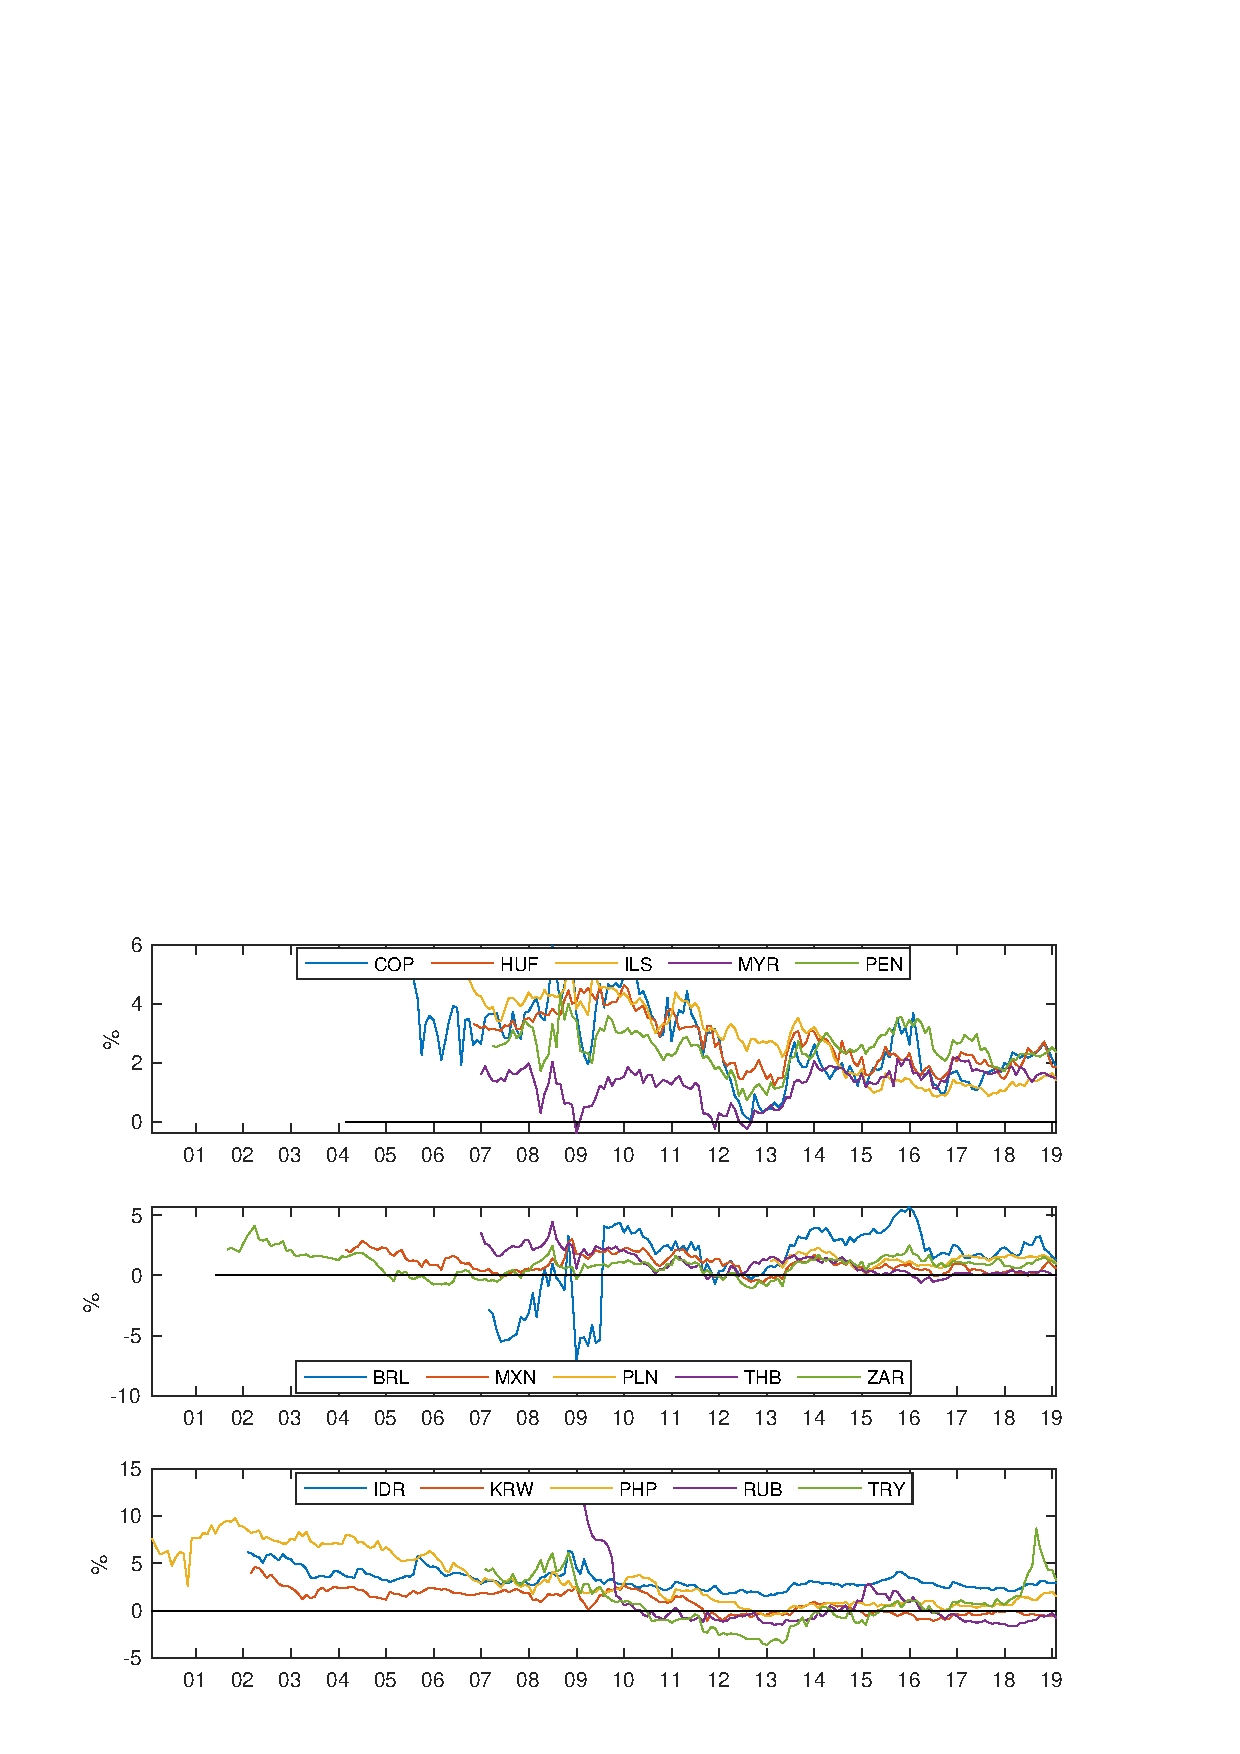
\includegraphics[width=1\textwidth,height=0.7\textheight]{../Figures/Temp/temp_tp10yrEM}
			\par\end{centering}
		\caption{Estimated 10-Year Term Premia: Emerging Markets.}\label{fig:temp_tp10yrEM}
	\end{figure}

Special cases include that of Brazil whose term premium turn negative around the Great Recession and that of Russia whose term premium declined considerably. These cases might be reflecting local conditions and deserve further analysis. Consider, for example, the case of Turkey towards the end of the sample, where relevant events in 2018\footnote{On June 24, 2018, Recep Tayyip Erdogan won the presidential election. On October 2, 2018, the journalist Jamal Khashoggi disappeared after he visited the consulate of Saudi Arabia in Istanbul.} translated into a higher term premium.

 In addition to Brazil, Russia and Turkey, the term premia of most Asian countries has been in negative territory for some period of time. Moreover, with the exception of Brazil and South Africa, the term premia of emerging markets being negative is a phenomenon observed after the Great Recession.

%To summarize the figure, Table \ref{tab:rp_stats} shows the mean of the 5-year synthetic yields and summary statistics for the estimated 5-year term premia. The means of the synthetic yields fluctuate between $2.3\%$ and $10.5\%$, while the means of the risk premia fluctuate between $-36$ basis points to $150$ basis points. On average, the term premium represents around $12\%$ of the synthetic 5-year yield. For Indonesia, Russia, South Africa and Turkey the standard deviation of their term premia is relatively high compared to their mean. Philippines and Russia had periods with a really negative term premia in October 2000 and the first half of 2015, respectively; excluding those episodes, the term premium has fluctuated between $-3.5\%$ and $5.5\%$.
%	\begin{table}
	\centering
\begin{tabular}{l|cccccc}
\toprule
\multicolumn{1}{c}{}& &\textbf{Yield}&\multicolumn{4}{c}{\textbf{Risk Premium}}\\
\cmidrule(l{.9em}r{.9em}){4-7}
%\cmidrule(lr){3}  \cmidrule(lr){4-7}
\multicolumn{1}{c}{}&\textbf{Obs}&\textbf{Mean}&\textbf{Mean}&\textbf{Std}&\textbf{Min}&\textbf{Max}\\\midrule
{ COP}&154&6.23&1.33&1.21&-0.96&4.41\\\
{HUF}&138&3.71&0.31&0.67&-0.95&1.50\\\
{IDR}&205&8.97&0.52&1.03&-3.06&3.92\\\
{ILS}&146&2.35&1.01&0.63&0.23&2.78\\\
{MXN}&173&6.22&0.88&0.74&-0.62&2.41\\\
{PEN}&141&4.64&1.50&1.55&-3.46&5.54\\\
{PHP}&219&6.54&1.21&1.25&-11.34&3.69\\\
{PLN}&157&3.33&0.64&0.52&-0.61&1.80\\\
{TRY}&155&10.52&-0.36&1.34&-3.22&2.29\\\
{KRW}&219&3.00&0.54&0.72&-1.09&3.51\\\
{MYR}&136&2.67&0.36&0.43&-0.66&1.31\\\
{RUB}&144&7.87&-0.13&1.88&-8.87&3.90\\\
{THB}&137&2.40&0.64&0.79&-1.03&2.89\\\
{ZAR}&218&8.38&0.45&1.12&-3.02&2.25\\ \bottomrule
\end{tabular}
\\
\caption{Summary Statistics: 5-Year Yield and Risk Premium.}\label{tab:rp_stats}
\end{table}

For comparison purposes, Figure \ref{fig:temp_tp10yrAE} shows the 10-year term premia estimates for advanced economies using synthetic yield curves. A clear downward trend is observed for all countries. This is consistent with the empirical evidence that uses nominal yield curves; \cite{Wright:2011} shows a declining trend in term premia for most of these countries going back to the 1990s and argues that it reflects a reduction in inflation uncertainty.
		\begin{figure}[!htbp]
		\begin{centering}
			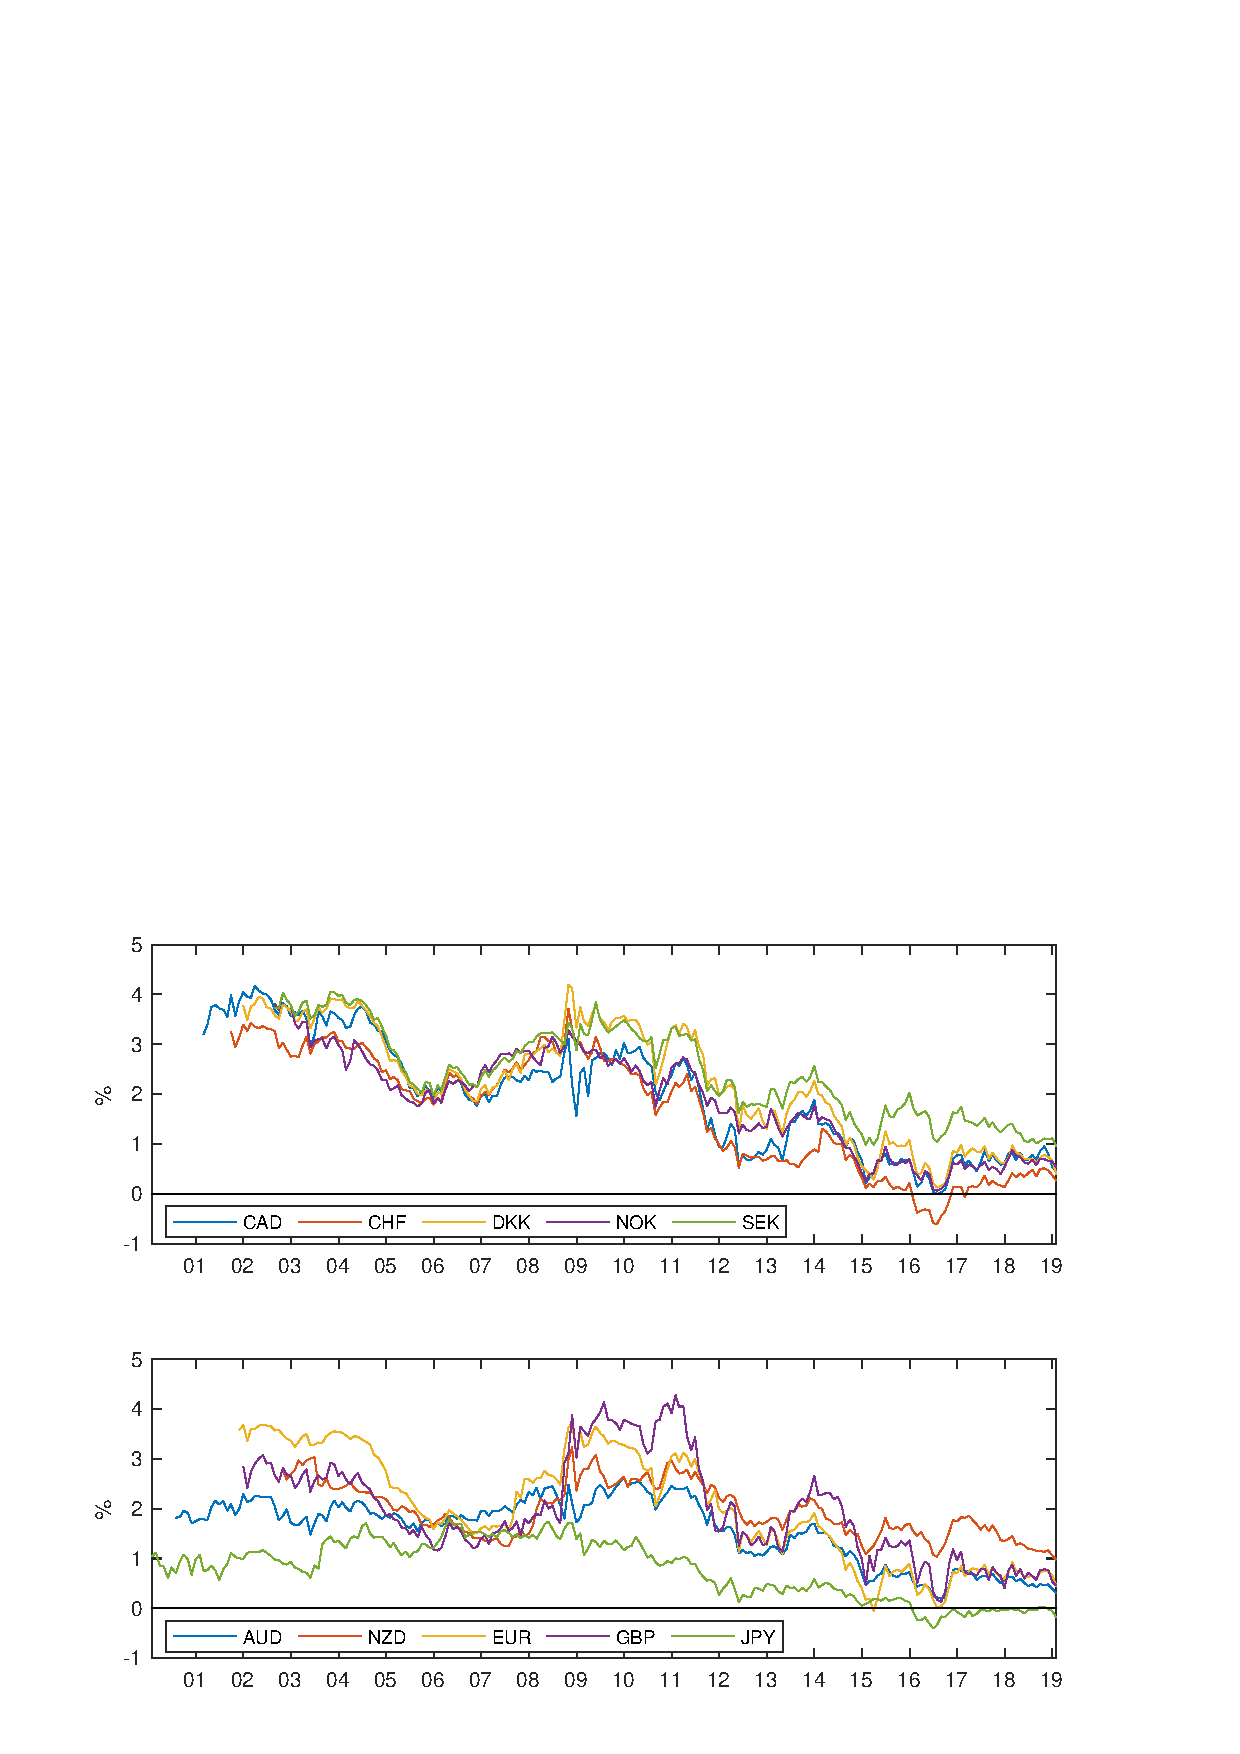
\includegraphics[width=1\textwidth,height=0.45\textheight]{../Figures/Temp/temp_tp10yrAE}
			\par\end{centering}
		\caption{Estimated 10-Year Term Premia: Advanced Economies.}\label{fig:temp_tp10yrAE}
	\end{figure}

Note that although the term premia of most advanced countries seem to reflect a common factor, that of Japan behaves differently probably reflecting the fact that Japan was at the zero lower bound before the other countries.

According to KW, the 10-year term premium estimate for the U.S. has been negative for most of the time since mid-2011, fluctuating between $-1$\% and $0$. Of the advanced countries considered, only Switzerland and Japan have experienced more than one month with a negative term premium, compared to several emerging markets, mainly Korea, Russia and Turkey. In particular, before the taper tantrum there was a tendency of declining term premia for emerging markets, which for some countries actually turned out negative.

\subsubsection{Term Structure of Term Premia}
In addition to comparing the term premia across countries, one can also compare them across maturities per country. In general, the term premium increases with maturity. As one would expect, when long-term bonds are seen as riskier than short-term bonds, investors would require a higher compensation for holding long-term bonds. This pattern, however, is not universal as can be seen in Figure \ref{fig:temp_ts_tp} in the Appendix, which shows two examples of this, namely Korea and Mexico. Therefore, the exceptions for the general pattern are observed in both emerging and advanced countries since the KW estimates also show that after the Great Recession, the 1-year U.S. term premium has been above the 5- and 10-year term premia at some points.
%\footnote{Sometimes, the standard deviation of the term premia increases with maturity.}
%		\begin{figure}[!htbp]
		\begin{centering}
			\vspace{12.5mm}
			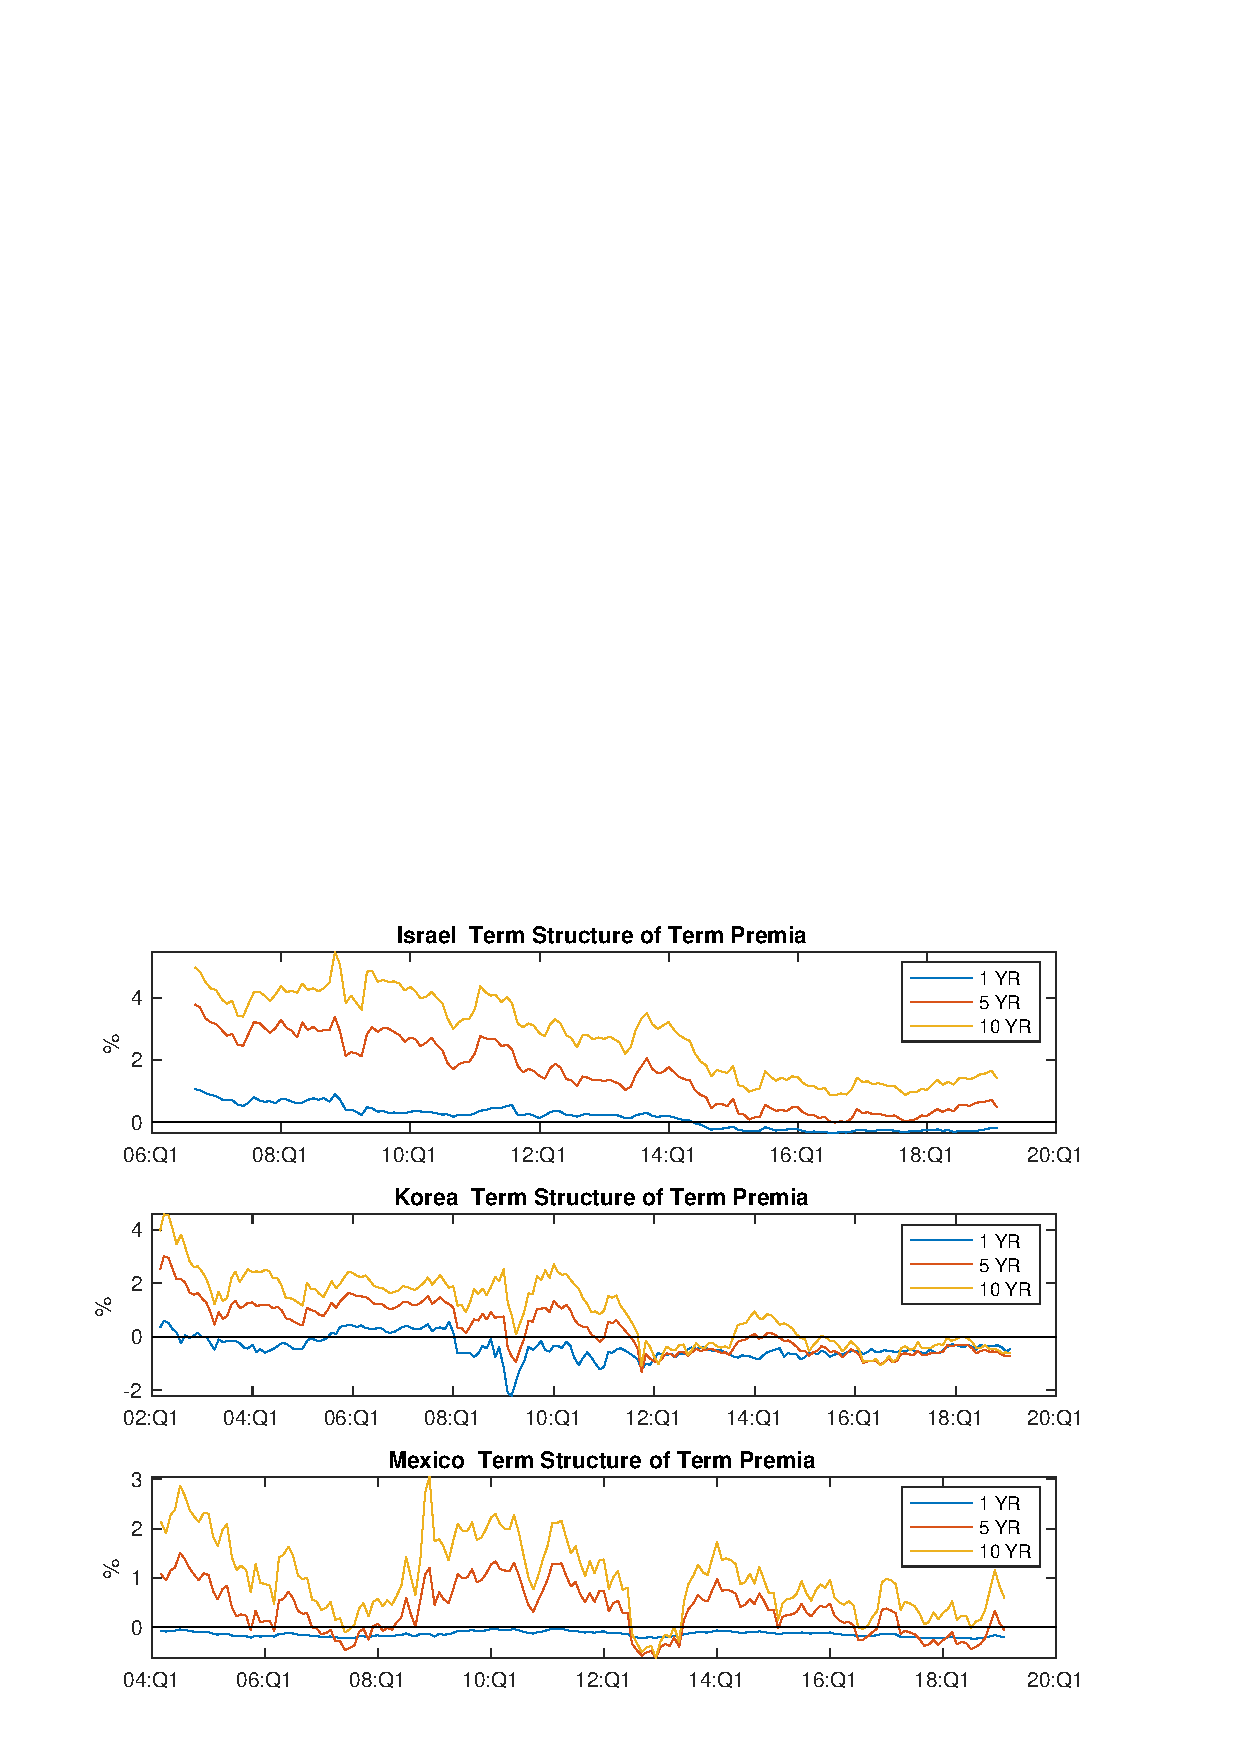
\includegraphics[width=1\textwidth,height=0.8\textheight]{../Figures/Temp/temp_ts_tp}
			\par\end{centering}
		\caption{Estimated Term Premia for Different Maturities.}\label{fig:temp_ts_tp}
	\end{figure}

\subsubsection{Common Factors in Term Premia}
To see whether there are common factors influencing the term premia in emerging markets, Table \ref{tab:temp_tp_common} shows the proportion of the total variation in the 10-year term premia explained by their first three PCs. To consider all countries, the starting date is December 2006. The first three PCs explain more than $80\%$ of the variation in the term premia of emerging markets and more than $98\%$ for advanced countries. This evidence highlights the importance of considering global factors as drivers of the term premia. But at the same time, the evidence for emerging markets shows that both domestic and common factors seem to be at play as drivers of their term premia.
%	\begin{table}
	\centering
\begin{tabular}{l|cccc}
\toprule
&\textbf{PC1}&\textbf{PC2}&\textbf{PC3}&\textbf{Sum}\\\midrule
{ Since Nov 2016} - All Countries&40.29&23.62&12.37&76.28\\\
Since Jun 2005 - 8 countries&52.46&16.66&12.08&81.19\\ \bottomrule
\end{tabular}
\\
\caption{Proportion of Total Variance in 5yr RP Explained by First 3 PCs.}
\label{tab:pc_common}
\end{table}

%	\begin{footnotesize}\begin{table}\centering\begin{tabular}{l|cccc}
\toprule
\multicolumn{1}{c}{} &\multicolumn{2}{c}{EM TP}&\multicolumn{2}{c}{Residual}\\
\cmidrule(l{1.1em}r{1.1em}){2-3} \cmidrule(l{1.1em}r{1.1em}){4-5}
\multicolumn{1}{c}{} & 5 YR & 10 YR & 5 YR & 10 YR \\
\midrule
(15) Dec-06 & 67.40 & 71.67 & 62.99 & 58.25 \\(8)  Jul-05 & 79.57 & 82.65 & 74.36 & 76.40 \\(4)  Latam & 95.43 & 94.96 & 94.01 & 92.47 \\(5)  Asia & 90.19 & 91.43 & 88.52 & 87.98 \\(4)  Europe & 97.38 & 95.25 & 97.15 & 93.38 \\\bottomrule\end{tabular}\caption{Percent of Total Variance Explained by First 3 PCs.}\label{table:CmnFctrs}\end{table}\end{footnotesize}
	\begin{tiny}\begin{table}\centering\begin{tabular}{l|cc}\toprule & Dec-2006 \\\midrule EM & 81.01 \\AE & 98.07 \\\bottomrule\end{tabular}\caption{Total Variation Explained by First 3 PCs (\%): 10-Year Term Premium.}\label{tab:temp_tp_common}\end{table}\end{tiny}

\subsubsection{Survey-Based Term Premia}
As already mentioned, one way to check the term premia estimates obtained from affine term structure models is to use survey data since long-term surveys of professional forecasters can be used to obtain a model-free estimate of the long-term term premium. Using this approach, the term premium is calculated as the difference between the long-term interest rate and the survey-expectation of the future short-term interest rate over the same horizon. Since the long-term expectations of the policy rate for emerging markets are not provided by Consensus Economics, they are approximated as explained in section \ref{sec:SurveyData}. As it is also explained in that section, given the persistence of bond yields, surveys can also provide information to help in the identification of the term premium.
 It is important to acknowledge, however, that surveys might not represent the market expectations or the expectations of the marginal investor.

Figure \ref{fig:temp_tp10yrSvy} displays the 10-year (long-term) term premium estimated in this way for most of the emerging markets considered in Figure \ref{fig:temp_tp10yrEM}.
		\begin{figure}[!htbp]
		\begin{centering}
			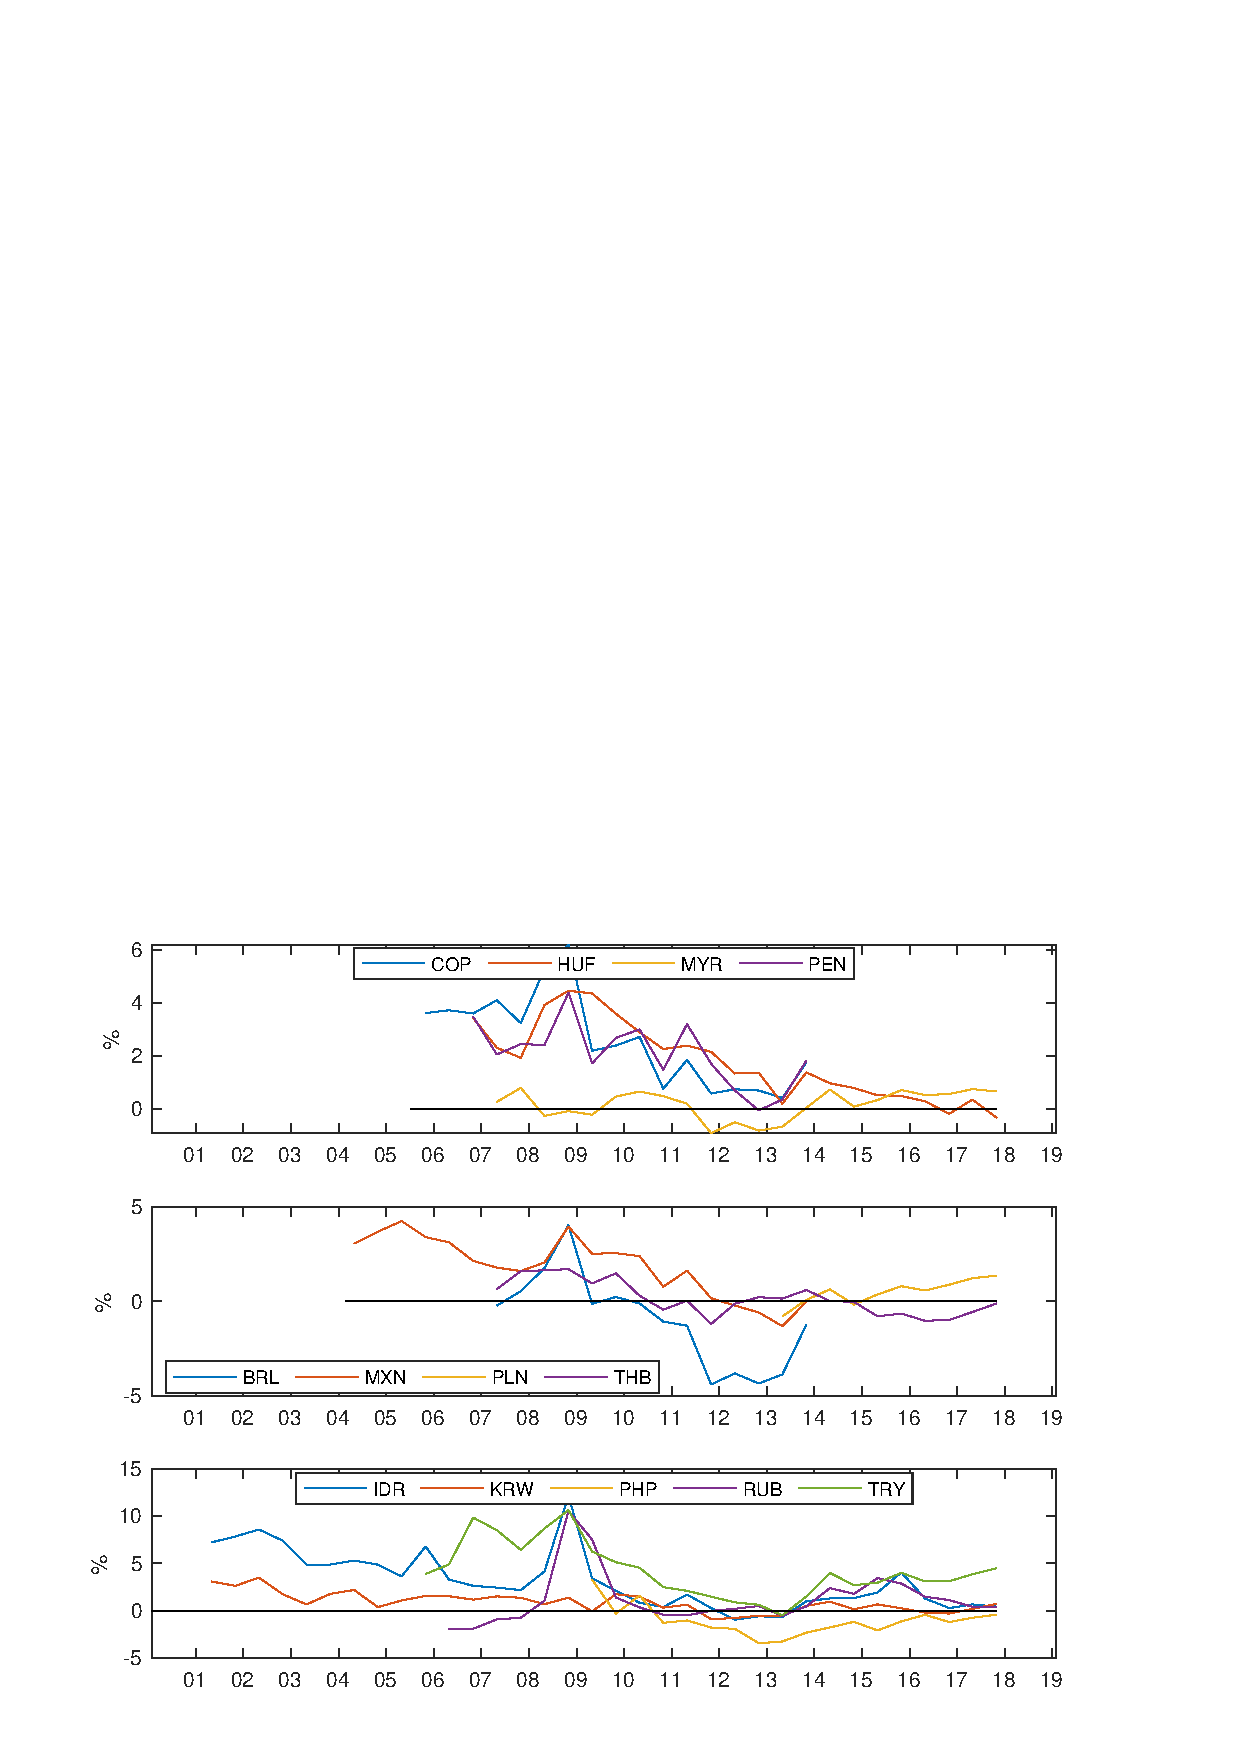
\includegraphics[width=1\textwidth,height=0.5\textheight]{../Figures/Temp/temp_tp10yrSvy}
			\par\end{centering}
		\caption{Survey-Based 10-Year Term Premium Estimates}\label{fig:temp_tp10yrSvy}
	\end{figure}

With the exception of Brazil during 2012-13, the term premia estimated using survey data are in line with the model-based term premia. In fact, the average correlation between the two is $80.4\%$.\footnote{Even for the term premia calculated using the nominal yield curve, the correlation with the survey-based term premia is equal to $85\%$.} This is reassuring and supports the idea of supplementing the term structure model with survey data to better pin down the term premia in emerging markets, which will in turn provide a more robust decomposition of the nominal yield curve. This will be done in future versions of this paper.

}{}	% Closes \iftoggle{fulldraft}


\section{International Spillovers of U.S. Monetary Policy} \label{sec:spillovers}
\iftoggle{toclinks}{\gototoc}{} % Turn it on/off in packages.tex, command in macros.tex
\iftoggle{cboxes}{	   				  % Turn it on/off in packages.tex
	\begin{boxeditems}
		\item Constrast the reference to Anaya et al. 2017 with Gilchrist, Yue \& Zakrajzek (2018) and with Wright et al. (2017).
		\item Contrast effect of FX with Hofman, Shim and Shin
		\item Claims about effect of variables on expected part can be tested using the expected part directly as well as forecasts.
	\end{boxeditems}}{}

Since this is the first time that term premia is estimated using synthetic yield curves, I first present their correlation with variables commonly associated with risk and uncertainty before proceeding to a more formal analysis.

\iftoggle{fulldraft}{					% Turn it on/off in packages.tex

%\subsection{Correlation with Financial Variables}
%Table \ref{tab:rp_reg_lvix} reports the regression of the term premia on $\ln \left( VIX \right)$. As it can be seen, the VIX plays a relevant role as the effect is significant for most of the countries. With the exception of Hungary and Malaysia, an increase in the VIX is associated with an increase in the term premia in emerging markets: a $10\%$ increase in the VIX increases the term premia by $10$ basis points on average. Based on the $R^2$, it explains more than $10\%$ of the variation in term premia for the countries for which the effect is higher.
%
%The effect of the federal funds rate is shown in Table \ref{tab:rp_reg_ffr}. It is significant in half of the countries. With the exception of Russia, an increase in the fed funds rate decreases the term premia by 25 basis points on average. It also explains more than $10\%$ of the variation in term premia for those countries. This is consistent with a flattening of the synthetic yield curve. Along with evidence that the monetary policy stance in emerging markets tend to move in the same direction than that in the U.S. \citep*{AnayaHachulaOffermanns:2017}, this is consistent with an increase in the expectation of future short-term interest rates in emerging markets.
%
%The exchange rate has an effect on the term premia of only four countries: Indonesia, Peru, Philippines and Russia. The results are reported in Table \ref{tab:rp_reg_rfx}. A $1\%$ depreciation of the LC is associated with a decrease in the term premia of 15 basis points on average for those countries. Along with the uncovered interest parity (according to which a LC depreciation would be followed by an increase in the short-term interest rate), this effect is also consistent with an increase in the expectation of future short-term interest rates.
%
%Unlike the previous financial variables, the return of the local stock market is not correlated with the term premia as shown in Table \ref{tab:rp_reg_stx}.\footnote{Since the countries studied are emerging markets, the return on the price of a commodity was also used as a regressor (in this case oil) but there was also no observed effect (not reported here).}

\subsection{Relationship with Risk and Uncertainty Measures}
To see how the term premia co-moves with variables associated with risk and uncertainty, they are compared against the 10-year U.S. term premium from KW, the LC credit spread from \cite{DuSchreger:2016JoF} or the convenience yield from \cite{DuImSchreger:2018JIE}, and the economic policy uncertainty (EPU) index proposed by \citet*{BakerBloomDavis:2016}. The first variable is an indicator of global financial conditions, while the second is an indicator of credit risk for emerging markets or the convenience yield for advanced economies. The EPU index is based on the frequency of articles in local newspapers containing key words such as `economy', `uncertainty' and `central bank'; however, it is only available for 5 of the emerging markets in the sample. Tables \ref{tab:temp_tp_corr10yr} and \ref{tab:temp_tp_corr10yr_epu} show these correlations.
%	\begin{tiny}\begin{table}\centering\begin{tabular}{l|ccc}\toprule & US TP & LCCS & EPU \\\midrule BRL & 0.38 & - & -0.29 \\COP & 0.67 & 0.09 & 0.13 \\HUF & 0.01 & -0.27 & - \\IDR & 0.36 & -0.21 & - \\ILS & 0.75 & -0.16 & - \\MXN & 0.72 & 0.20 & -0.05 \\PEN & 0.63 & -0.34 & - \\PHP & 0.49 & -0.22 & - \\PLN & 0.58 & -0.12 & - \\TRY & 0.76 & -0.16 & - \\KRW & 0.59 & 0.02 & -0.07 \\MYR & 0.23 & -0.53 & - \\RUB & 0.46 & -0.46 & -0.47 \\THB & 0.57 & -0.76 & - \\ZAR & 0.21 & 0.15 & - \\\bottomrule\end{tabular}\caption{Correlations of 10-Year Term Premia.}\label{table:Correls10yr}\end{table}\end{tiny}
	\begin{tiny}\begin{table}\centering\begin{tabular}{l|ccc}\toprule & TP-USTP & TP-CIP Dev & $\perp$TP-CIP Dev \\\midrule EM & 0.60 & -0.28 & -0.13 \\A-SOE & 0.80 & -0.01 & -0.20 \\G-3 & 0.71 & -0.29 & -0.22 \\\bottomrule\end{tabular}\caption{Correlations of 10-Year Term Premia: U.S TP and LCCS.}\label{tab:temp_tp_corr10yr}\end{table}\end{tiny}
	\begin{tiny}\begin{table}
		\centering
		\begin{tabular}{l|ccccc}
			\toprule
			 & BRL & COP & KRW & MXN & RUB \\
			 \midrule 
			 TP-EPU & 0.14 & 0.46 & -0.32 & 0.40 & -0.22 \\
%			 $\perp$TP-EPU & 0.11 & 0.28 & -0.31 & 0.20 & -0.09 \\
			 \bottomrule
		 \end{tabular}
	 \caption{Correlations of 10-Year Term Premia: Economic Policy Uncertainty Index}\label{tab:temp_tp_corr10yr_epu}\end{table}\end{tiny}

The term premia in emerging markets is related to the U.S. term premium but not as tightly linked as those for advanced countries. To assess the relationship of the country-specific component of the term premia with the other two variables, I regress the term premium of each country on the U.S. term premium and use the residuals as the `idiosyncratic' term premium (i.e. the part of a country's term premium orthogonal to the U.S. term premium).

The correlation of the term premia with the deviations from CIP is negative. \cite{DuSchreger:2016JoF} show that the LC credit spread has a low reaction to global variables. This provides a possible explanation for the negative relationship between the term premia and the LC credit spread, since the former seems to react to global factors as is formally tested in the next section. The last column of table \ref{tab:temp_tp_corr10yr}  shows that once the term premia in emerging markets is purged from the effect of the U.S. term premium, the relationship is still negative but the magnitude declines. The opposite is observed for advanced small open economies but remember that for them the deviations from CIP reflect a convenience yield.

The term premia for Latin American countries show a positive correlation with the EPU index; the correlation for Korea and Russia, however, is negative. The relationship might be related to the fact that after the Great Recession, the term premia for both countries has been negative during a considerable period as shown in figure \ref{fig:temp_tp10yrEM}. This can be verified if the EPU index for countries with a similar situation (like Turkey) becomes available. Although the magnitude declines, the sign of the relationship with the idiosyncratic component of the term premia holds suggesting a role for domestic drivers of the term premia.

%\subsection{Correlation with Macroeconomic Variables}
%Three variables that are closely followed by market participants are inflation, the unemployment rate and industrial production because they capture the state of the economy at a monthly frequency. Therefore, the macroeconomic variables used in this section are the year-on-year percentage change in the consumer price index, the unemployment rate and the year-on-year percentage change in industrial production in each country. All countries have at least two of the three variables available for their respective time span, and only seven countries have the three variables available during their whole sample period.\footnote{The seven countries are Colombia, Hungary, Korea, Mexico, Peru, Russia and Turkey. Inflation is not included for Philippines since it is available starting in January 2013. Unemployment is not included for Israel (available since January 2012), Poland (March 2010) and South Africa (March 2008). Industrial production is not included for Indonesia (January 2011), Malaysia (January 2013) and Thailand (February 2011).} 
%
%The available macroeconomic variables are included in the regressions at the same time. The results are reported in Table \ref{tab:rp_reg_macro}. The table shows that inflation and the unemployment rate are important drivers of the term premia. They are significant for all countries for which they are included. An increase in inflation tends to decrease the term premia by 12 basis points on average, while unemployment increases term premia by 50 basis points on average. These effects are consistent with an active monetary policy in line with the standard textbook mechanism and expectations of future short-term interest rates following the same direction of the policy rate. Industrial production is important statistically and economically only for Peru.
%
%In addition, the variation in term premia explained by these variables is relatively high, $34\%$ on average, which is higher than for any of the financial variables analyzed before. This supports including macroeconomic factors in the vector of state variables. In future versions, this can be done following \citet*{JPS:2014}, which will also help in further testing the relevance of unspanned or hidden factors in emerging markets.

\subsection{Drivers of Term Premia}
To study the cyclical properties of term premia in emerging markets formally, I run  panel data regressions with a variety of macroeconomic and financial variables as explanatory variables. The macroeconomic variables considered have a monthly frequency; for the financial variables considered (which are available daily) end-of-month values are used.

The panel data regressions have the form
	\begin{equation} \label{eq:panelTPreg}
	\eqpanelTPreg .
\end{equation}

\noindent where $tp_{it}$ denotes the model-based 10-year term premium of country $i$ in month $t$, $z_{it}$ is a vector of regressors and $\alpha_{i}$ denotes country fixed effects. The regressors include global and domestic variables as suggested by the evidence presented in tables \ref{tab:temp_tp_common}-\ref{tab:temp_tp_corr10yr_epu}. This is a first step towards understanding the drivers of term premia and, therefore, it is important to acknowledge the potential econometric problems such as endogeneity as well as the effects of the persistence of the variables considered.

The global financial variables include the Cboe's volatility index (VIX), the federal funds rate, the S\&P $500$ index and the oil price. The VIX and the federal funds rate have been used in the global financial cycle literature \citep[see][]{Rey:2013} to study the effects of common factors on capital flows. The VIX is usually used as a measure of risk aversion and economic uncertainty and the fed funds rate is a measure of the monetary policy stance in the U.S. Given the sudden spikes in the VIX, it is common to use the $\ln \left( VIX \right)$ instead of the VIX directly. For the U.S. monetary policy, the variable used is the effective federal funds rate calculated by the New York Fed. 
 
 The domestic variables include inflation, the unemployment rate and industrial production to capture macroeconomic effects. In addition, the exchange rate (LC per USD) and the local stock market index are used as measures of local financial conditions. 
 
 Monthly returns, calculated as the log difference of the series, are used for the stock market indexes, the oil price and the exchange rate.

Table \ref{tab:temp_tp_regs} reports different specifications of the model in equation (\ref{eq:panelTPreg}). The first model in the table focuses mainly on global variables, while the second one focuses on domestic variables. These two models already shed some light on the driving forces behind the term premia in emerging markets. However, the models with the most explanatory power include both global and domestic variables.
%	\begin{tiny}\begin{tabular}{cccccc}
\toprule
log(VIX)& 0.021&-0.195&& 0.538***& 0.513***\\\
 &(0.33)&(0.32)&&(0.15)&(0.14)\\\
FFR&-0.198***& 0.009&&-0.149*& 0.109\\\
 &(0.08)&(0.08)&&(0.08)&(0.09)\\\
USTP10&& 0.546***&&& 0.639***\\\
 &&(0.06)&&&(0.06)\\\
SPX&-0.001***&-0.000&&-0.001***&\\\
 &(0.00)&(0.00)&&(0.00)&\\\
INF&&&-0.090&-0.136**&-0.150**\\\
 &&&(0.07)&(0.06)&(0.05)\\\
UNE&&& 0.160& 0.047& 0.029\\\
 &&&(0.12)&(0.10)&(0.09)\\\
IP&&&-0.008& 0.002&-0.001\\\
 &&&(0.01)&(0.01)&(0.01)\\\
Country FE&Yes&Yes&Yes&Yes&Yes\\\
Observations&2483&2483&1757&1757&1757\\\
Countries&15&15&15&15&15\\\
Within $R^2$&0.15&0.23&0.07&0.26&0.38\\\
\end{tabular}
\end{tiny}
	% Preview source code for paragraph 0
\begin{scriptsize}
% Preview source code for paragraph 0
\begin{table}
\begin{center}
\begin{tabular}{lr@{\extracolsep{0pt}.}lr@{\extracolsep{0pt}.}lr@{\extracolsep{0pt}.}lr@{\extracolsep{0pt}.}lr@{\extracolsep{0pt}.}lr@{\extracolsep{0pt}.}l}
	\hline 
 & \multicolumn{2}{c}{(1)} & \multicolumn{2}{c}{(2)} & \multicolumn{2}{c}{(3)} & \multicolumn{2}{c}{(4)} & \multicolumn{2}{c}{(5)} & \multicolumn{2}{c}{(6)}\tabularnewline
	\hline 
	& \multicolumn{2}{c}{} & \multicolumn{2}{c}{} & \multicolumn{2}{c}{} & \multicolumn{2}{c}{} & \multicolumn{2}{c}{} & \multicolumn{2}{c}{}\tabularnewline
	log(VIX) & 0&20 & \multicolumn{2}{c}{} & 0&26 & 0&24 & 0&65{*}{*}{*} & 0&10\tabularnewline
	& (0&35) & \multicolumn{2}{c}{} & (0&24) & (0&16) & (0&21) & (0&19)\tabularnewline
	FFR & 0&07 & \multicolumn{2}{c}{} & 0&23{*}{*} & 0&13 & 0&22{*}{*} & 0&11\tabularnewline
	& (0&11) & \multicolumn{2}{c}{} & (0&09) & (0&09) & (0&10) & (0&10)\tabularnewline
	USTP10 & 1&49{*}{*}{*} & \multicolumn{2}{c}{} & \multicolumn{2}{c}{} & 1&30{*}{*}{*} & \multicolumn{2}{c}{} & 1&22{*}{*}{*}\tabularnewline
	& (0&20) & \multicolumn{2}{c}{} & \multicolumn{2}{c}{} & (0&12) & \multicolumn{2}{c}{} & (0&16)\tabularnewline
	S\&P & -0&00 & \multicolumn{2}{c}{} & -0&00{*} & \multicolumn{2}{c}{} & \multicolumn{2}{c}{} & \multicolumn{2}{c}{}\tabularnewline
	& (0&00) & \multicolumn{2}{c}{} & (0&00) & \multicolumn{2}{c}{} & \multicolumn{2}{c}{} & \multicolumn{2}{c}{}\tabularnewline
	Oil & -0&01{*} & \multicolumn{2}{c}{} & 0&00 & \multicolumn{2}{c}{} & \multicolumn{2}{c}{} & \multicolumn{2}{c}{}\tabularnewline
	& (0&01) & \multicolumn{2}{c}{} & (0&00) & \multicolumn{2}{c}{} & \multicolumn{2}{c}{} & \multicolumn{2}{c}{}\tabularnewline
	Inflation & \multicolumn{2}{c}{} & 0&26{*}{*}{*} & 0&19{*}{*}{*} & 0&19{*}{*}{*} & 0&22{*}{*}{*} & 0&21{*}{*}{*}\tabularnewline
	& \multicolumn{2}{c}{} & (0&05) & (0&06) & (0&05) & (0&05) & (0&05)\tabularnewline
	Unemployment & \multicolumn{2}{c}{} & 0&21{*}{*}{*} & 0&17{*}{*} & 0&13{*}{*} & 0&21{*}{*}{*} & 0&13{*}{*}\tabularnewline
	& \multicolumn{2}{c}{} & (0&07) & (0&06) & (0&05) & (0&06) & (0&05)\tabularnewline
	IP & \multicolumn{2}{c}{} & -0&01 & -0&01 & -0&02 & -0&02 & -0&02{*}\tabularnewline
	& \multicolumn{2}{c}{} & (0&01) & (0&01) & (0&01) & (0&01) & (0&01)\tabularnewline
	zFX & \multicolumn{2}{c}{} & 0&21{*} & 0&41{*}{*} & 0&29{*}{*} & \multicolumn{2}{c}{} & \multicolumn{2}{c}{}\tabularnewline
	& \multicolumn{2}{c}{} & (0&11) & (0&15) & (0&10) & \multicolumn{2}{c}{} & \multicolumn{2}{c}{}\tabularnewline
	Stock Market & \multicolumn{2}{c}{} & -0&00{*}{*} & -0&00 & -0&00 & \multicolumn{2}{c}{} & \multicolumn{2}{c}{}\tabularnewline
	& \multicolumn{2}{c}{} & (0&00) & (0&00) & (0&00) & \multicolumn{2}{c}{} & \multicolumn{2}{c}{}\tabularnewline
	Return S\&P & \multicolumn{2}{c}{} & \multicolumn{2}{c}{} & \multicolumn{2}{c}{} & \multicolumn{2}{c}{} & 0&00 & -0&01\tabularnewline
	& \multicolumn{2}{c}{} & \multicolumn{2}{c}{} & \multicolumn{2}{c}{} & \multicolumn{2}{c}{} & (0&01) & (0&01)\tabularnewline
	Return Oil & \multicolumn{2}{c}{} & \multicolumn{2}{c}{} & \multicolumn{2}{c}{} & \multicolumn{2}{c}{} & 0&00 & 0&00\tabularnewline
	& \multicolumn{2}{c}{} & \multicolumn{2}{c}{} & \multicolumn{2}{c}{} & \multicolumn{2}{c}{} & (0&00) & (0&00)\tabularnewline
	Return FX & \multicolumn{2}{c}{} & \multicolumn{2}{c}{} & \multicolumn{2}{c}{} & \multicolumn{2}{c}{} & 0&02{*} & 0&01\tabularnewline
	& \multicolumn{2}{c}{} & \multicolumn{2}{c}{} & \multicolumn{2}{c}{} & \multicolumn{2}{c}{} & (0&01) & (0&01)\tabularnewline
	Return Stocks & \multicolumn{2}{c}{} & \multicolumn{2}{c}{} & \multicolumn{2}{c}{} & \multicolumn{2}{c}{} & 0&00 & 0&00\tabularnewline
	& \multicolumn{2}{c}{} & \multicolumn{2}{c}{} & \multicolumn{2}{c}{} & \multicolumn{2}{c}{} & (0&01) & (0&01)\tabularnewline
	Constant & 2&01 & -0&65 & -0&44 & -1&03 & -3&18{*}{*}{*} & -0&73\tabularnewline
	& (1&66) & (0&63) & (1&41) & (0&85) & (0&93) & (0&80)\tabularnewline
	& \multicolumn{2}{c}{} & \multicolumn{2}{c}{} & \multicolumn{2}{c}{} & \multicolumn{2}{c}{} & \multicolumn{2}{c}{} & \multicolumn{2}{c}{}\tabularnewline
	Observations & \multicolumn{2}{c}{2,407} & \multicolumn{2}{c}{1,969} & \multicolumn{2}{c}{1,969} & \multicolumn{2}{c}{1,969} & \multicolumn{2}{c}{1,969} & \multicolumn{2}{c}{1,969}\tabularnewline
	R-squared & 0&32 & 0&32 & 0&39 & 0&53 & 0&34 & 0&49\tabularnewline
	Number of Countries & \multicolumn{2}{c}{15} & \multicolumn{2}{c}{15} & \multicolumn{2}{c}{15} & \multicolumn{2}{c}{15} & \multicolumn{2}{c}{15} & \multicolumn{2}{c}{15}\tabularnewline
	Country FE & \multicolumn{2}{c}{Yes} & \multicolumn{2}{c}{Yes} & \multicolumn{2}{c}{Yes} & \multicolumn{2}{c}{Yes} & \multicolumn{2}{c}{Yes} & \multicolumn{2}{c}{Yes}\tabularnewline
	\hline 
	\multicolumn{13}{l}{Robust standard errors in parentheses; {*}{*}{*} p$<$0.01, {*}{*} p$<$0.05,
		{*} p$<$0.1.}\tabularnewline
\end{tabular}\caption{Panel Data Regressions of the 10-Year Term Premium (\%).} \label{tab:temp_tp_regs}
\end{center}
\end{table}
\end{scriptsize}


The main global factor is the U.S. term premium, and the two main domestic factors are inflation and unemployment. Holding the other factors constant, an increase in any of these three variables increases the term premia in emerging markets. Note that external conditions have a relevant impact on domestic bond markets since the greatest effect comes from the U.S. term premium. This is in line with the literature studying the global financial cycle that focuses on capital flows. However, the channel does not seem to be through the VIX nor even through the monetary policy of the U.S. directly via the federal funds rate but through the U.S. term premia. Both the VIX and the federal funds rate appear to have a positive effect on the term premia in emerging markets but the effect disappears once the U.S. term premium is included in the regressions. An increase in the U.S. term premium translates into a more than proportional increase in the term premium of emerging markets.

The effect of the domestic variables is in line with what has been found for advanced countries using nominal yield curves. Investors demand a higher term premium during recessions, when the unemployment rate increases. This provides evidence of a countercyclical behavior of the term premia in emerging markets. Moreover, the positive effect of inflation on the term premia conforms with the idea that inflation erodes the value of nominal bonds and so in periods of rising inflation investors demand a higher term premium. The effect of both variables is broadly similar across models. 

The exchange rate also seems to be playing a role; a depreciation of the local currency is associated with an increase in the term premium. This seems counterintuitive from the perspective of the standard trade-channel effect since emerging markets are usually commodity exporters. However, it is in line with the risk-taking channel of exchange rates found by \cite{HofmannShimShin:2017}, according to which currency appreciation is associated with easier financial conditions and compressed sovereign bond spreads.

Finally, the effects of the domestic variables remain once one controls for time fixed effects. The effects of those variables remain broadly similar across the different specifications.

}{}	% Closes \iftoggle{fulldraft}


\section{Concluding Remarks}\label{sec:conclusions}
\iftoggle{toclinks}{\gototoc}{} % Turn it on/off in packages.tex, command in macros.tex
\iftoggle{cboxes}{	   				  % Turn it on/off in packages.tex
	\begin{boxeditems}
		\item Study how the effect of macroeconomic and financial variables on the term premia compare to their effect on the LC credit spread and on the expectation of future short-term interest rates. That is, perform a full decomposition of `observed' yields (default risk, term premia and expectations of future short-term interest rates) and analyze the effects of said variables on each component. This would extend the analysis done by GilchristYueZakrajsek:2019 on the spillover effects of U.S. monetary policy on LC bonds of emerging markets. Compare also with HofmannShimShin:2017. The set of variables could be extended too (e.g. monetary policy shocks in other advanced economies).
		\item Perform a more robust analysis of the determinants of term premia in emerging markets and how they differ from those of advanced economies.
		\item Uncovered interest parity is based on risk-neutrality. Could the risk-neutral yields obtained from the term structure model be used to revisit the findings from the literature on deviations from uncovered interest parity for EMs? This will extend the work done by AngChen:2010.
		\item Can the findings from this research be used to make a decomposition of the FC-denominated yield curve? Following the same strategy of using synthetic yield curves. Similar to the way it can be done for the U.S. yield curve, the FC yield curve can be swapped into LC, which would allow a comparison between the FC and the LC yield curves. Can this be related to exchange rates and inflation expectations? To sovereign risks?
		\item The estimated yield curves are an input to the decomposition of the changes in the exchange rates (risk premia, inflation expectations) done by StavrakevaTang:2018b for advanced economies, which could be extended for emerging markets.
		\item Exploit the cross-section of yields by using a multi-country term structure model in order to improve the precision in the term premia estimates. In future versions, a multi-country affine term structure model may be used in the spirit of JotikasthiraLeLundblad:2015 to exploit information in the cross-section of yield curves.
		\item Forecast the LC yields in emerging markets.
	\end{boxeditems}}{}

%The analysis in this paper provides insights into the dynamics of the yield curves in emerging markets.

The sovereign yields of emerging markets comove. I use synthetic yield curve to account for credit risk, which allows me to decompose the nominal yield curves of 15 emerging markets into three three parts: an expectation for the future short-term interest rate, a term premium and a credit risk premium. The comovement in sovereign yields is mainly driven by the term premia.

\iftoggle{fulldraft}{					% Turn it on/off in packages.tex

%This paper estimates the term premia for 15 emerging markets using synthetic yield curves. The LC credits spread accounts for the difference between the nominal and the synthetic yield curve. By accounting for credit risk, this paper avoids violating the risk-free assumption underlying affine term structure models.
%Exploiting the flexibility of these models, I decompose the synthetic yield curve into an expectation for the future short-term interest rate and a term premium, which in turn allows to decompose the nominal yield curve into three components (the third one being the LC credit spread).

%The evidence presented shows that the main component for the 10-year yield of emerging markets is the expected future path of the short-term interest rate, while for advanced economies the main component is the term premium. 
The term premia in emerging markets for the 10-year maturity is around 175 basis points on average, more than double the size of the credit risk premium. 
%higher than the average of the LC credit spread of 85 basis points
The results are compared to those obtained from surveys of professional forecasters and from advanced countries to establish a set of stylized facts. 
%It is shown that the 
There are benefits of using synthetic yield curves. 
%are greater for emerging markets than for advanced economies, which implies that the terms `risk premium' and `term premium' should not be used interchangeably, at least for emerging markets. The analysis also shows that 
For instance, the phenomenon of a negative term premium is not limited to advanced countries.
%The analysis shows that both 
Furthermore, global and domestic factors are important drivers of the term premia in emerging markets. The U.S. term premium is a key common factor having a more than proportional effect on their term premia. The evidence also shows a countercyclical behavior of the term premia as well as a positive relationship with inflation, in line with the idea that it erodes the value of nominal bonds.

The work presented in this paper can be extended in several directions and I will continue working on them. First, as already indicated, the information from survey data can aid in mitigating the identification problem in affine term structure models, which translates into more robust estimates of the term premia. As a consequence, the decomposition of the nominal yield curve will also be more robust so that it can provide useful information for the analysis of monetary policy in emerging markets.

Different models can also be used to assess different characteristics of the data from the synthetic curves. A model that explicitly considers the joint behavior of nominal and real interest rates can allow to further decompose both nominal and synthetic yield curves into the expectation of the future real interest rate and the real term premium. The model can also be supplemented not only with survey data but also with macroeconomic information. Other extensions include models with jumps in yields, which might be applicable to a couple of emerging markets (those with a poor fit mentioned in section \ref{sec:results}). Given the reaction to common factors, multi-country term structure models might be relevant. To further study the phenomenon of negative term premiums, quadratic term structure models with joint dynamics for stocks and bonds might be useful.

Finally, other improvements can also be included like extending the comparison with advanced economies for the analysis shown in section \ref{sec:spillovers}. In particular, analyzing the relationship between the EPU index for those advanced countries for which it is available (Australia, Canada, Germany, Japan, UK and Sweden) to compare it with what is reported for emerging markets, as well as contrasting the results from the panel regressions to advanced countries. More generally, the panel regression analysis can be applied to the other components of the nominal yield curve, namely the expectation part and the LC credit spread. This will provide a broader picture of the relative importance of global and domestic factors on local bond markets.

}{}	% Closes \iftoggle{fulldraft}


%---------------------------------------------------------------
% Figures and Tables
%---------------------------------------------------------------

%\newpage
%\input{../Figures/fig1}	% \ref{fig:fig1}
%\input{../Tables/tab1}		% \ref{tab:tab1}